% Options for packages loaded elsewhere
\PassOptionsToPackage{unicode}{hyperref}
\PassOptionsToPackage{hyphens}{url}
\PassOptionsToPackage{dvipsnames,svgnames,x11names}{xcolor}
%
\documentclass[
  letterpaper,
  DIV=11,
  numbers=noendperiod]{scrartcl}

\usepackage{amsmath,amssymb}
\usepackage{iftex}
\ifPDFTeX
  \usepackage[T1]{fontenc}
  \usepackage[utf8]{inputenc}
  \usepackage{textcomp} % provide euro and other symbols
\else % if luatex or xetex
  \usepackage{unicode-math}
  \defaultfontfeatures{Scale=MatchLowercase}
  \defaultfontfeatures[\rmfamily]{Ligatures=TeX,Scale=1}
\fi
\usepackage{lmodern}
\ifPDFTeX\else  
    % xetex/luatex font selection
\fi
% Use upquote if available, for straight quotes in verbatim environments
\IfFileExists{upquote.sty}{\usepackage{upquote}}{}
\IfFileExists{microtype.sty}{% use microtype if available
  \usepackage[]{microtype}
  \UseMicrotypeSet[protrusion]{basicmath} % disable protrusion for tt fonts
}{}
\makeatletter
\@ifundefined{KOMAClassName}{% if non-KOMA class
  \IfFileExists{parskip.sty}{%
    \usepackage{parskip}
  }{% else
    \setlength{\parindent}{0pt}
    \setlength{\parskip}{6pt plus 2pt minus 1pt}}
}{% if KOMA class
  \KOMAoptions{parskip=half}}
\makeatother
\usepackage{xcolor}
\setlength{\emergencystretch}{3em} % prevent overfull lines
\setcounter{secnumdepth}{-\maxdimen} % remove section numbering
% Make \paragraph and \subparagraph free-standing
\ifx\paragraph\undefined\else
  \let\oldparagraph\paragraph
  \renewcommand{\paragraph}[1]{\oldparagraph{#1}\mbox{}}
\fi
\ifx\subparagraph\undefined\else
  \let\oldsubparagraph\subparagraph
  \renewcommand{\subparagraph}[1]{\oldsubparagraph{#1}\mbox{}}
\fi

\usepackage{color}
\usepackage{fancyvrb}
\newcommand{\VerbBar}{|}
\newcommand{\VERB}{\Verb[commandchars=\\\{\}]}
\DefineVerbatimEnvironment{Highlighting}{Verbatim}{commandchars=\\\{\}}
% Add ',fontsize=\small' for more characters per line
\usepackage{framed}
\definecolor{shadecolor}{RGB}{241,243,245}
\newenvironment{Shaded}{\begin{snugshade}}{\end{snugshade}}
\newcommand{\AlertTok}[1]{\textcolor[rgb]{0.68,0.00,0.00}{#1}}
\newcommand{\AnnotationTok}[1]{\textcolor[rgb]{0.37,0.37,0.37}{#1}}
\newcommand{\AttributeTok}[1]{\textcolor[rgb]{0.40,0.45,0.13}{#1}}
\newcommand{\BaseNTok}[1]{\textcolor[rgb]{0.68,0.00,0.00}{#1}}
\newcommand{\BuiltInTok}[1]{\textcolor[rgb]{0.00,0.23,0.31}{#1}}
\newcommand{\CharTok}[1]{\textcolor[rgb]{0.13,0.47,0.30}{#1}}
\newcommand{\CommentTok}[1]{\textcolor[rgb]{0.37,0.37,0.37}{#1}}
\newcommand{\CommentVarTok}[1]{\textcolor[rgb]{0.37,0.37,0.37}{\textit{#1}}}
\newcommand{\ConstantTok}[1]{\textcolor[rgb]{0.56,0.35,0.01}{#1}}
\newcommand{\ControlFlowTok}[1]{\textcolor[rgb]{0.00,0.23,0.31}{#1}}
\newcommand{\DataTypeTok}[1]{\textcolor[rgb]{0.68,0.00,0.00}{#1}}
\newcommand{\DecValTok}[1]{\textcolor[rgb]{0.68,0.00,0.00}{#1}}
\newcommand{\DocumentationTok}[1]{\textcolor[rgb]{0.37,0.37,0.37}{\textit{#1}}}
\newcommand{\ErrorTok}[1]{\textcolor[rgb]{0.68,0.00,0.00}{#1}}
\newcommand{\ExtensionTok}[1]{\textcolor[rgb]{0.00,0.23,0.31}{#1}}
\newcommand{\FloatTok}[1]{\textcolor[rgb]{0.68,0.00,0.00}{#1}}
\newcommand{\FunctionTok}[1]{\textcolor[rgb]{0.28,0.35,0.67}{#1}}
\newcommand{\ImportTok}[1]{\textcolor[rgb]{0.00,0.46,0.62}{#1}}
\newcommand{\InformationTok}[1]{\textcolor[rgb]{0.37,0.37,0.37}{#1}}
\newcommand{\KeywordTok}[1]{\textcolor[rgb]{0.00,0.23,0.31}{#1}}
\newcommand{\NormalTok}[1]{\textcolor[rgb]{0.00,0.23,0.31}{#1}}
\newcommand{\OperatorTok}[1]{\textcolor[rgb]{0.37,0.37,0.37}{#1}}
\newcommand{\OtherTok}[1]{\textcolor[rgb]{0.00,0.23,0.31}{#1}}
\newcommand{\PreprocessorTok}[1]{\textcolor[rgb]{0.68,0.00,0.00}{#1}}
\newcommand{\RegionMarkerTok}[1]{\textcolor[rgb]{0.00,0.23,0.31}{#1}}
\newcommand{\SpecialCharTok}[1]{\textcolor[rgb]{0.37,0.37,0.37}{#1}}
\newcommand{\SpecialStringTok}[1]{\textcolor[rgb]{0.13,0.47,0.30}{#1}}
\newcommand{\StringTok}[1]{\textcolor[rgb]{0.13,0.47,0.30}{#1}}
\newcommand{\VariableTok}[1]{\textcolor[rgb]{0.07,0.07,0.07}{#1}}
\newcommand{\VerbatimStringTok}[1]{\textcolor[rgb]{0.13,0.47,0.30}{#1}}
\newcommand{\WarningTok}[1]{\textcolor[rgb]{0.37,0.37,0.37}{\textit{#1}}}

\providecommand{\tightlist}{%
  \setlength{\itemsep}{0pt}\setlength{\parskip}{0pt}}\usepackage{longtable,booktabs,array}
\usepackage{calc} % for calculating minipage widths
% Correct order of tables after \paragraph or \subparagraph
\usepackage{etoolbox}
\makeatletter
\patchcmd\longtable{\par}{\if@noskipsec\mbox{}\fi\par}{}{}
\makeatother
% Allow footnotes in longtable head/foot
\IfFileExists{footnotehyper.sty}{\usepackage{footnotehyper}}{\usepackage{footnote}}
\makesavenoteenv{longtable}
\usepackage{graphicx}
\makeatletter
\def\maxwidth{\ifdim\Gin@nat@width>\linewidth\linewidth\else\Gin@nat@width\fi}
\def\maxheight{\ifdim\Gin@nat@height>\textheight\textheight\else\Gin@nat@height\fi}
\makeatother
% Scale images if necessary, so that they will not overflow the page
% margins by default, and it is still possible to overwrite the defaults
% using explicit options in \includegraphics[width, height, ...]{}
\setkeys{Gin}{width=\maxwidth,height=\maxheight,keepaspectratio}
% Set default figure placement to htbp
\makeatletter
\def\fps@figure{htbp}
\makeatother

\KOMAoption{captions}{tableheading}
\makeatletter
\makeatother
\makeatletter
\makeatother
\makeatletter
\@ifpackageloaded{caption}{}{\usepackage{caption}}
\AtBeginDocument{%
\ifdefined\contentsname
  \renewcommand*\contentsname{Table of contents}
\else
  \newcommand\contentsname{Table of contents}
\fi
\ifdefined\listfigurename
  \renewcommand*\listfigurename{List of Figures}
\else
  \newcommand\listfigurename{List of Figures}
\fi
\ifdefined\listtablename
  \renewcommand*\listtablename{List of Tables}
\else
  \newcommand\listtablename{List of Tables}
\fi
\ifdefined\figurename
  \renewcommand*\figurename{Figure}
\else
  \newcommand\figurename{Figure}
\fi
\ifdefined\tablename
  \renewcommand*\tablename{Table}
\else
  \newcommand\tablename{Table}
\fi
}
\@ifpackageloaded{float}{}{\usepackage{float}}
\floatstyle{ruled}
\@ifundefined{c@chapter}{\newfloat{codelisting}{h}{lop}}{\newfloat{codelisting}{h}{lop}[chapter]}
\floatname{codelisting}{Listing}
\newcommand*\listoflistings{\listof{codelisting}{List of Listings}}
\makeatother
\makeatletter
\@ifpackageloaded{caption}{}{\usepackage{caption}}
\@ifpackageloaded{subcaption}{}{\usepackage{subcaption}}
\makeatother
\makeatletter
\@ifpackageloaded{tcolorbox}{}{\usepackage[skins,breakable]{tcolorbox}}
\makeatother
\makeatletter
\@ifundefined{shadecolor}{\definecolor{shadecolor}{rgb}{.97, .97, .97}}
\makeatother
\makeatletter
\makeatother
\makeatletter
\makeatother
\ifLuaTeX
  \usepackage{selnolig}  % disable illegal ligatures
\fi
\IfFileExists{bookmark.sty}{\usepackage{bookmark}}{\usepackage{hyperref}}
\IfFileExists{xurl.sty}{\usepackage{xurl}}{} % add URL line breaks if available
\urlstyle{same} % disable monospaced font for URLs
\hypersetup{
  pdftitle={1. Introduction},
  colorlinks=true,
  linkcolor={blue},
  filecolor={Maroon},
  citecolor={Blue},
  urlcolor={Blue},
  pdfcreator={LaTeX via pandoc}}

\title{1. \protect\hyperlink{toc0_}{Introduction}}
\author{}
\date{}

\begin{document}
\maketitle
\ifdefined\Shaded\renewenvironment{Shaded}{\begin{tcolorbox}[enhanced, boxrule=0pt, frame hidden, interior hidden, borderline west={3pt}{0pt}{shadecolor}, breakable, sharp corners]}{\end{tcolorbox}}\fi

Stellar Physics - Part 1: Stellar Properties

Dr Rosaria Lena

Room 620, Kelvin Building

\href{mailto:rosaria.lena@glasgow.ac.uk}{\nolinkurl{rosaria.lena@glasgow.ac.uk}}

\begin{center}\rule{0.5\linewidth}{0.5pt}\end{center}

\textbf{Table of contents}\\
- 1. \protect\hyperlink{toc1_}{Introduction}\\
- 1.1. \protect\hyperlink{toc1_1_}{Look at the night sky, what do we
see?}\\
- 2. \protect\hyperlink{toc2_}{What is a star?}\\
- 2.1. \protect\hyperlink{toc2_1_}{Life and death of a star}\\
- 2.2. \protect\hyperlink{toc2_2_}{Do all stars look the same?}\\
- 2.3. \protect\hyperlink{toc2_3_}{A comparison between two stars on
Stellarium}\\
- 2.4. \protect\hyperlink{toc2_4_}{What can we tell from
observations?}\\
- 3. \protect\hyperlink{toc3_}{How distant are the stars?}\\
- 3.1. \protect\hyperlink{toc3_1_}{An easy case: the distance to the
Sun}\\
- 3.2. \protect\hyperlink{toc3_2_}{The astronomical unit}\\
- 3.2.1. \protect\hyperlink{toc3_2_1_}{Question}\\
- 3.2.2. \protect\hyperlink{toc3_2_2_}{A remark on the Astronomical
Unit}\\
- 3.3. \protect\hyperlink{toc3_3_}{Size of our solar system}\\
- 3.4. \protect\hyperlink{toc3_4_}{How do we measure the distance to the
stars?}\\
- 3.4.1. \protect\hyperlink{toc3_4_1_}{The parallax method}\\
- 3.4.2. \protect\hyperlink{toc3_4_2_}{The nearest star: Proxima
Centauri}\\
- 3.4.3. \protect\hyperlink{toc3_4_3_}{`Spot the mistake' question:}\\
- 3.5. \protect\hyperlink{toc3_5_}{Transit method}\\
- 4. \protect\hyperlink{toc4_}{How big are stars?}\\
- 4.1. \protect\hyperlink{toc4_1_}{How big is the Sun?}\\
- 4.2. \protect\hyperlink{toc4_2_}{What about other stars?}\\
- 4.2.1. \protect\hyperlink{toc4_2_1_}{A comparison of some star
sizes}\\
- 4.3. \protect\hyperlink{toc4_3_}{A handy guide to estimating angular
diameters}\\
- 4.4. \protect\hyperlink{toc4_4_}{How far apart are the stars?}\\
- 5. \protect\hyperlink{toc5_}{How bright are stars?}\\
- 5.1. \protect\hyperlink{toc5_1_}{Apparent brightness and luminosity}\\
- 5.1.1. \protect\hyperlink{toc5_1_1_}{The Sun's luminosity}\\
- 5.1.2. \protect\hyperlink{toc5_1_2_}{`Spot the mistake' question}\\
- 5.2. \protect\hyperlink{toc5_2_}{Stellar magnitude scales}\\
- 5.2.1. \protect\hyperlink{toc5_2_1_}{Apparent magnitude}\\
- 5.2.1.1. \protect\hyperlink{toc5_2_1_1_}{Apparent magnitude zero point
convention}\\
- 5.2.1.2. \protect\hyperlink{toc5_2_1_2_}{~Question}\\
- 5.2.2. \protect\hyperlink{toc5_2_2_}{Magnitude and units}\\
- 5.2.3. \protect\hyperlink{toc5_2_3_}{Absolute Magnitude}\\
- 5.2.3.1. \protect\hyperlink{toc5_2_3_1_}{Absolute magnitude zero point
convention}\\
- 5.2.4. \protect\hyperlink{toc5_2_4_}{Question}\\
- 5.2.5. \protect\hyperlink{toc5_2_5_}{Relationship between apparent
magnitude and absolute magnitude}\\
- 5.3. \protect\hyperlink{toc5_3_}{Apparent magnitude and luminosity}\\
- 5.4. \protect\hyperlink{toc5_4_}{Absolute magnitude and luminosity}\\
- 5.5. \protect\hyperlink{toc5_5_}{Magnitudes, luminosity and
distance}\\
- 5.6. \protect\hyperlink{toc5_6_}{Example}\\
- 5.7. \protect\hyperlink{toc5_7_}{Note on types of magnitude}\\
- 5.8. \protect\hyperlink{toc5_8_}{Setting the Absolute Magnitude
scale}\\
- 6. \protect\hyperlink{toc6_}{Recap}\\
- 7. \protect\hyperlink{toc7_}{Stellar Colour}\\
- 7.1.1. \protect\hyperlink{toc7_1_1_}{Why are the stars different
colours?}\\
- 7.2. \protect\hyperlink{toc7_2_}{Black body radiation}\\
- 7.2.1. \protect\hyperlink{toc7_2_1_}{Rayleigh-Jeans law}\\
- 7.2.2. \protect\hyperlink{toc7_2_2_}{Wien's law}\\
- 7.3. \protect\hyperlink{toc7_3_}{Planck's Law}\\
- 7.3.1. \protect\hyperlink{toc7_3_1_}{Exercise:}\\
- 8. \protect\hyperlink{toc8_}{Temperature and colour}\\
- 8.1. \protect\hyperlink{toc8_1_}{Wien's displacement law}\\
- 8.2. \protect\hyperlink{toc8_2_}{Example}\\
- 8.3. \protect\hyperlink{toc8_3_}{(!) Converting between wavelength and
frequency}\\
- 8.4. \protect\hyperlink{toc8_4_}{Okay, but how big is an a.u.?}\\
- 8.5. \protect\hyperlink{toc8_5_}{Are stars really black bodies?}\\
- 9. \protect\hyperlink{toc9_}{Stefan-Boltzmann Law}\\
- 10. \protect\hyperlink{toc10_}{Stellar luminosity}\\
- 10.1. \protect\hyperlink{toc10_1_}{Example}\\
- 11. \protect\hyperlink{toc11_}{Recap}

Astronomy is a \emph{observational} science. We cannot bring a star down
to Earth to study it in the laboratory. Unlike other branches of
Physics, we cannot experiment directly on stars and what happens in the
universe is beyond our control, but we can use our knowledge of Physics
to make predictions and we can use observations to validate our
theories. This can allow us to answer many questions about the stars.
Some of these questions date back to the most ancient times, and through
history have inspired philosophers and scientists to develop our
understanding of the cosmos. This interplay between Astronomy and
Physics is today called \emph{Astrophysics}, which has grown to
encompass phenomena from planets to galaxies to the evolution of the
universe.

\textbf{Astrophysics is very multidisciplinary}

\begin{figure}

{\centering 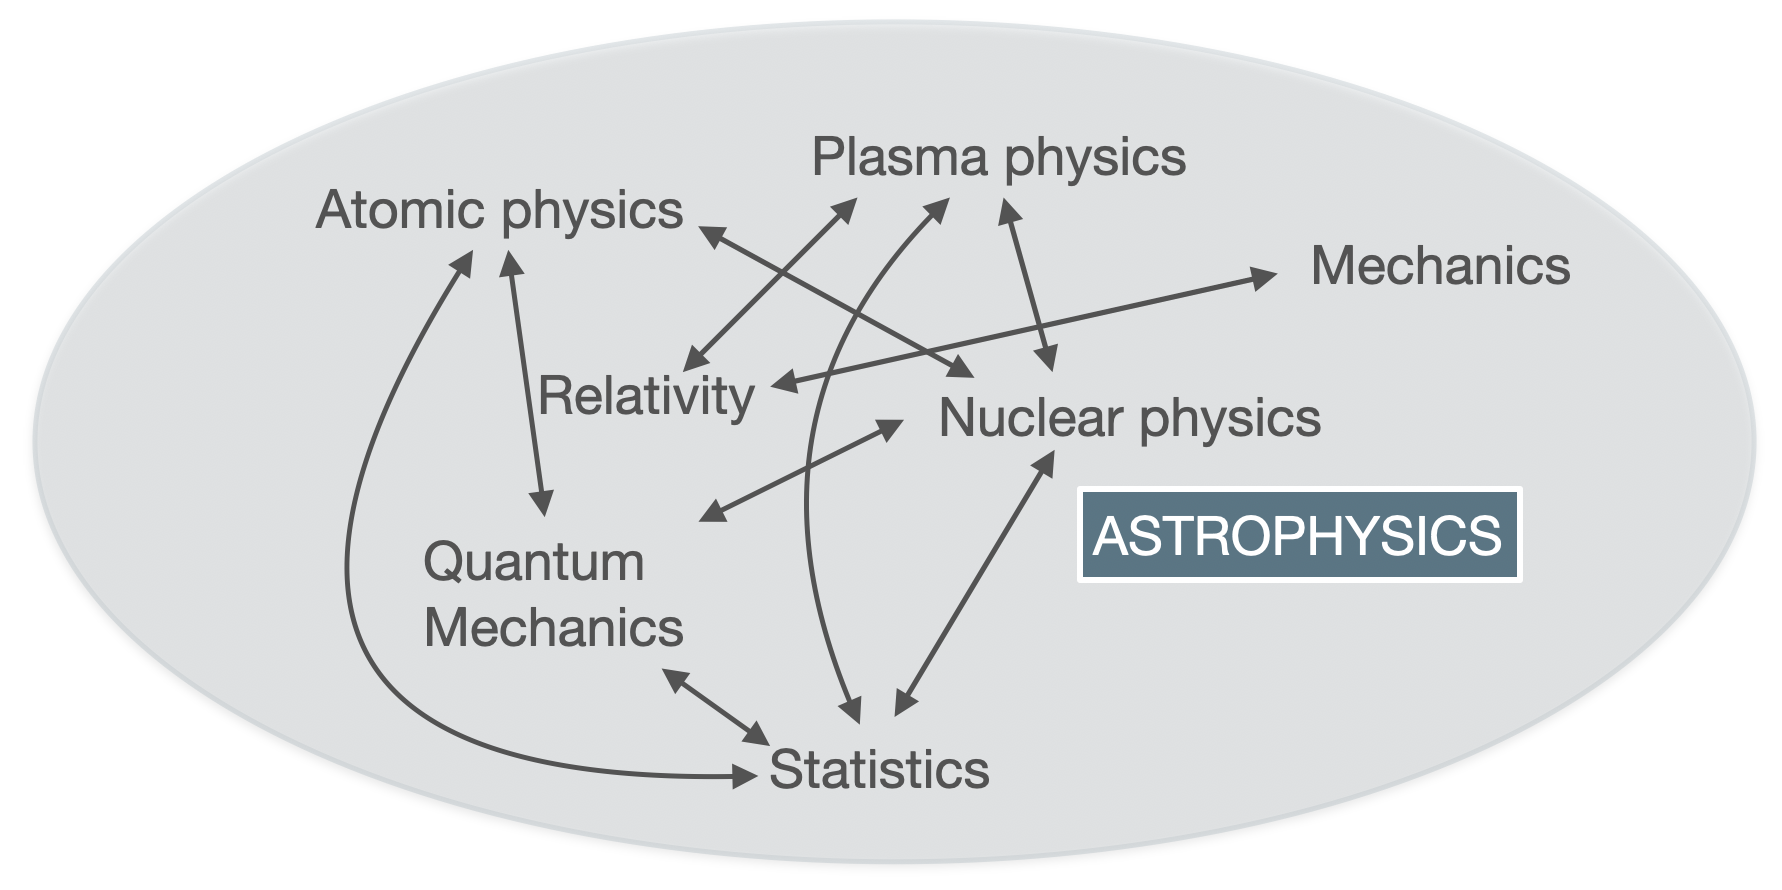
\includegraphics{img/astrophysics_multidisciplinary.png}

}

\caption{Multidisciplinarity in astrophysics}

\end{figure}

Astrophysics is very multidisciplinary because of `several effects' that
come into play in the physics of stars, galaxies, the universe\ldots{}
it is an `arena' of different fields of physics (but also mathematics
and chemistry), spanning across classical mechanics, relativity, nuclear
and particle physics, statistics, atomic and molecular physics, plasma
physics, quantum mechanics and more (the list above and in the picture
is not exhaustive)! In this course you will see how some of these fields
play a role in the physics of stars.

\hypertarget{look-at-the-night-sky-what-do-we-see}{%
\subsection{\texorpdfstring{1.1. \protect\hyperlink{toc0_}{Look at the
night sky, what do we
see?}}{1.1. Look at the night sky, what do we see?}}\label{look-at-the-night-sky-what-do-we-see}}

Let's start with some simple observations of the night sky\ldots{}
``Look at the night sky, what do we see?'' Here in Scotland, the answer
to this questions is likely `clouds', but if you are curious to know
what is beyond those clouds, you can check out Stellarium (you can
download it or you can use the web version:
https://stellarium-web.org/).

All that glitters is not (only) stars!

\begin{figure}

{\centering \includegraphics{img/Stellarium_full.png}

}

\caption{An example from Stellarium}

\end{figure}

Looking at the night sky we may be able to see planets, meteors,
galaxies, satellites, comets, star clusters and many stars!

\begin{figure}

{\centering \includegraphics{img/Stellarium_full_description.png}

}

\caption{An example from Stellarium (with marked typical objects)}

\end{figure}

\hypertarget{what-is-a-star}{%
\section{\texorpdfstring{2. \protect\hyperlink{toc0_}{What is a
star?}}{2. What is a star?}}\label{what-is-a-star}}

A star is an astronomical spheroid body: - held together by
\emph{self-gravity} - \emph{radiating} energy from an internal source
(tipycally from nuclear fusion reactions, and occasionally from the
release of gravitational potential energy during contraction or
collapse)

Having this definition you should be able to answer this question: ``is
the Death Star a (fictional) star''?

The answer is ``no'', because it does not radiate energy! The Death Star
is actually a (fictional) space station orbiting the (fictional) planet
moon of Endor. Enough with the fictional stuff now.

If you look at the sky you may see that planets and comets are also
shining in the sky, so why can't they be considered stars, based on the
definition given above? Do they radiate energy? Are they
self-gravitating?

Planets actually do not \emph{radiate}, they mostly reflect the light
coming from the Sun, and the same holds for comets. In addition to that,
comets do not have enough mass to be considered self-gravitating
objects.

\hypertarget{life-and-death-of-a-star}{%
\subsection{\texorpdfstring{2.1. \protect\hyperlink{toc0_}{Life and
death of a
star}}{2.1. Life and death of a star}}\label{life-and-death-of-a-star}}

A star is not a static object. During its life it will evolve, changing
its internal structure and chemical composition as it `burns its
\emph{fuel}' and changing its mass and size, eventually resulting in its
death when one of the conditions that define a star is no longer valid,
i.e.~when the star is no longer self-gravitating or when it stops
radiating having exhausted its nuclear fuel. We will talk more about the
evolution of stars in the following lectures. Now let's go back to what
we can observe having a look at the night sky and let's see what we can
tell from observations of stars.

\hypertarget{do-all-stars-look-the-same}{%
\subsection{\texorpdfstring{2.2. \protect\hyperlink{toc0_}{Do all stars
look the
same?}}{2.2. Do all stars look the same?}}\label{do-all-stars-look-the-same}}

\begin{figure}

{\centering \includegraphics{img/M3_color3.gif}

}

\caption{M3}

\end{figure}

\begin{itemize}
\tightlist
\item
  There are a lot of stars, not uniformly distributed
\item
  Some look brighter than others
\item
  Some are bigger than others
\item
  They have different colours
\item
  Sometimes there are coloured or dark areas around stars
\item
  Some stars have fluctuating brightness: repeating and irregular
\end{itemize}

\hypertarget{a-comparison-between-two-stars-on-stellarium}{%
\subsection{\texorpdfstring{2.3. \protect\hyperlink{toc0_}{A comparison
between two stars on
Stellarium}}{2.3. A comparison between two stars on Stellarium}}\label{a-comparison-between-two-stars-on-stellarium}}

Let's check the properties of two stars on Stellarium. What can you
notice after a first look at these stars? You may notice that they have
different colours (one looks white, the other one looks white-blue). The
boxes contain some information about these stars, and you may recognise
many of these fields in the blue boxes from positional astronomy. We
will find out what the properties in the red boxes mean during this
course.

\begin{figure}

{\centering \includegraphics{img/Stellarium_stars_p.png}

}

\caption{Comparison between two stars on Stellarium}

\end{figure}

\hypertarget{what-can-we-tell-from-observations}{%
\subsection{\texorpdfstring{2.4. \protect\hyperlink{toc0_}{What can we
tell from
observations?}}{2.4. What can we tell from observations?}}\label{what-can-we-tell-from-observations}}

\begin{itemize}
\tightlist
\item
  How distant are the stars?
\item
  How big are they?
\item
  How bright?
\item
  How, when and where do they form?
\item
  What are their most important characteristics?
\item
  What are they made of?
\item
  What is their energy source?
\item
  What happens when it runs out?
\end{itemize}

\hypertarget{how-distant-are-the-stars}{%
\section{\texorpdfstring{3. \protect\hyperlink{toc0_}{How distant are
the
stars?}}{3. How distant are the stars?}}\label{how-distant-are-the-stars}}

\hypertarget{an-easy-case-the-distance-to-the-sun}{%
\subsection{\texorpdfstring{3.1. \protect\hyperlink{toc0_}{An easy case:
the distance to the
Sun}}{3.1. An easy case: the distance to the Sun}}\label{an-easy-case-the-distance-to-the-sun}}

\textbf{How do we find the distance to the Sun?}

Easy! - Just define The Astronomical Unit (a.u.) as the average distance
between the Earth and the Sun!

\hypertarget{the-astronomical-unit}{%
\subsection{\texorpdfstring{3.2. \protect\hyperlink{toc0_}{The
astronomical
unit}}{3.2. The astronomical unit}}\label{the-astronomical-unit}}

Ok, but how big is an au? In 1976 the International Astronomical Union
(IAU) adopted a standard definition whose value has been updated with
increasing precision during the years. At the current date, the
astronomical unit is: - 1 a.u. = 149,597,870,700 m

\hypertarget{question}{%
\subsubsection{\texorpdfstring{3.2.1.
\protect\hyperlink{toc0_}{Question}}{3.2.1. Question}}\label{question}}

Can you now work out how long it takes for the sunlight to reach Earth?

\begin{Shaded}
\begin{Highlighting}[]
\ImportTok{import}\NormalTok{ warnings}
\NormalTok{warnings.filterwarnings(}\StringTok{\textquotesingle{}ignore\textquotesingle{}}\NormalTok{)}
\ImportTok{import}\NormalTok{ math}
\NormalTok{AU }\OperatorTok{=} \DecValTok{149597870} \CommentTok{\# km}
\NormalTok{c }\OperatorTok{=} \FloatTok{299792.458} \CommentTok{\# km/s}
\NormalTok{ts }\OperatorTok{=}\NormalTok{ AU}\OperatorTok{/}\NormalTok{c }\CommentTok{\# s}
\NormalTok{tm }\OperatorTok{=}\NormalTok{ ts}\OperatorTok{/}\DecValTok{60} \CommentTok{\# min}
\BuiltInTok{print}\NormalTok{(}\SpecialStringTok{f"Time taken by light to reach Earth from the Sun = }\SpecialCharTok{\{}\NormalTok{ts}\SpecialCharTok{:1.4\}}\SpecialStringTok{ s = }\SpecialCharTok{\{}\NormalTok{tm}\SpecialCharTok{:1.4\}}\SpecialStringTok{ min = 8\textquotesingle{} 19\textquotesingle{}\textquotesingle{} "}\NormalTok{)}
\end{Highlighting}
\end{Shaded}

\begin{verbatim}
Time taken by light to reach Earth from the Sun = 499.0 s = 8.317 min = 8' 19'' 
\end{verbatim}

\hypertarget{a-remark-on-the-astronomical-unit}{%
\subsubsection{\texorpdfstring{3.2.2. \protect\hyperlink{toc0_}{A remark
on the Astronomical
Unit}}{3.2.2. A remark on the Astronomical Unit}}\label{a-remark-on-the-astronomical-unit}}

Note: 1 a.u. is an \emph{average} distance, because the distance between
the Earth and the Sun varies during the year.

\begin{Shaded}
\begin{Highlighting}[]
\ImportTok{import}\NormalTok{ warnings}
\NormalTok{warnings.filterwarnings(}\StringTok{\textquotesingle{}ignore\textquotesingle{}}\NormalTok{)}
\ImportTok{import}\NormalTok{ math}
\NormalTok{AU }\OperatorTok{=} \DecValTok{149597870} \CommentTok{\# km}
\NormalTok{aphD }\OperatorTok{=} \DecValTok{152100000} \CommentTok{\# km}
\NormalTok{perD }\OperatorTok{=} \DecValTok{147100000} \CommentTok{\# km}
\NormalTok{AU\_avg }\OperatorTok{=}\NormalTok{ (aphD}\OperatorTok{+}\NormalTok{perD)}\OperatorTok{/}\NormalTok{(}\DecValTok{2}\OperatorTok{*}\NormalTok{AU) }\CommentTok{\# Average distance, gives AU, check: print(f"\{AU\_avg\}")}
\BuiltInTok{print}\NormalTok{(}\SpecialStringTok{f"Distance Earth{-}Sun at aphelion (most distant) = }\SpecialCharTok{\{}\NormalTok{aphD}\SpecialCharTok{:1.3e\}}\SpecialStringTok{ km = }\SpecialCharTok{\{}\NormalTok{aphD}\OperatorTok{/}\NormalTok{AU}\SpecialCharTok{:1.4\}}\SpecialStringTok{ au"}\NormalTok{)}
\BuiltInTok{print}\NormalTok{(}\SpecialStringTok{f"Distance Earth{-}Sun at perihelion (closest) = }\SpecialCharTok{\{}\NormalTok{perD}\SpecialCharTok{:1.3e\}}\SpecialStringTok{ km = }\SpecialCharTok{\{}\NormalTok{perD}\OperatorTok{/}\NormalTok{AU}\SpecialCharTok{:1.3\}}\SpecialStringTok{ au"}\NormalTok{)}
\BuiltInTok{print}\NormalTok{(}\SpecialStringTok{f"Average distance Earth{-}Sun = }\SpecialCharTok{\{}\NormalTok{AU}\SpecialCharTok{:1.3e\}}\SpecialStringTok{ km = 1 au"}\NormalTok{)}
\end{Highlighting}
\end{Shaded}

\begin{verbatim}
Distance Earth-Sun at aphelion (most distant) = 1.521e+08 km = 1.017 au
Distance Earth-Sun at perihelion (closest) = 1.471e+08 km = 0.983 au
Average distance Earth-Sun = 1.496e+08 km = 1 au
\end{verbatim}

\begin{Shaded}
\begin{Highlighting}[]
\ImportTok{from}\NormalTok{ IPython.display }\ImportTok{import}\NormalTok{ display, HTML}
\NormalTok{display(HTML(}\StringTok{"\textless{}style\textgreater{}.container \{ width:100\% !important; \}\textless{}/style\textgreater{}"}\NormalTok{))}
\end{Highlighting}
\end{Shaded}

\begin{verbatim}
<IPython.core.display.HTML object>
\end{verbatim}

\hypertarget{size-of-our-solar-system}{%
\subsection{\texorpdfstring{3.3. \protect\hyperlink{toc0_}{Size of our
solar
system}}{3.3. Size of our solar system}}\label{size-of-our-solar-system}}

\begin{longtable}[]{@{}ll@{}}
\toprule\noalign{}
Planet & Distance from Sun (a.u.) \\
\midrule\noalign{}
\endhead
\bottomrule\noalign{}
\endlastfoot
Mercury & 0.39 \\
Venus & 0.72 \\
Earth & 1 \\
Mars & 1.52 \\
Jupiter & 5.20 \\
Saturn & 9.54 \\
Uranus & 19.2 \\
Neptune & 30.06 \\
\end{longtable}

\hypertarget{how-do-we-measure-the-distance-to-the-stars}{%
\subsection{\texorpdfstring{3.4. \protect\hyperlink{toc0_}{How do we
measure the distance to the
stars?}}{3.4. How do we measure the distance to the stars?}}\label{how-do-we-measure-the-distance-to-the-stars}}

\hypertarget{the-parallax-method}{%
\subsubsection{\texorpdfstring{3.4.1. \protect\hyperlink{toc0_}{The
parallax
method}}{3.4.1. The parallax method}}\label{the-parallax-method}}

We started with the easy example of answering how distant is the Sun,
but what about other stars? One way to determine the distance to nearest
stars is to use the \emph{parallax method}.

If you look at the position of a closer object against a further
background, you will notice that the image of the near object will shift
in the background as you move. This effect is called parallax and you
can experience it even when you close one eye at the time looking at an
object against a background.

\begin{figure}

{\centering 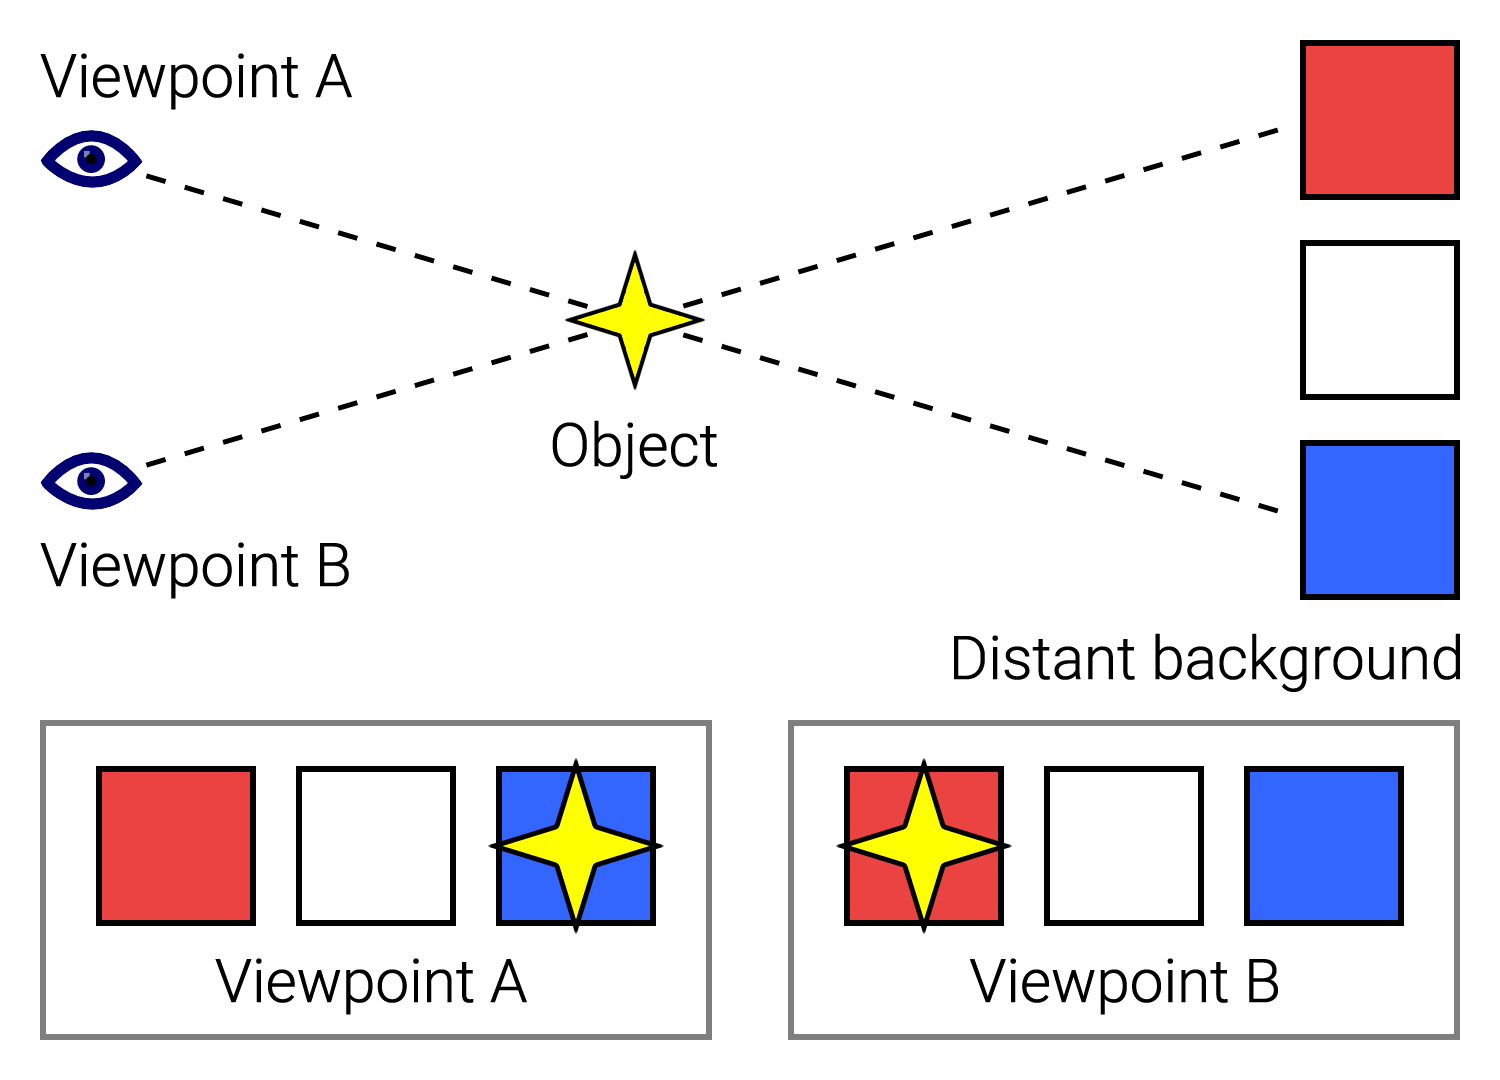
\includegraphics{img/Parallax_Example.png}

}

\caption{Parallax1}

\end{figure}

Analogously, in a background of distant stars, a closer star will appear
to move against them as the Earth orbits the Sun. So how do we use this
to determine the distance to a start? We use trigonometry.

The angle formed between the lines of sight of a star from two positions
of the observer is twice the parallax angle. In the example below, the
parallax is the angle between the lines of sight of the observer on
Earth and from the Sun (the middle point between the position of Earth
six months apart).

The number of stars that can be observed from Earth is limited and
nowadays \emph{direct} observations of the distance using the parallax
method are done by satellites orbiting the Sun in sync with Earth.
Hipparcos gathered data on more than one million stars, and its
successor Gaia has already observed 2 billion stars!

\begin{figure}

{\centering 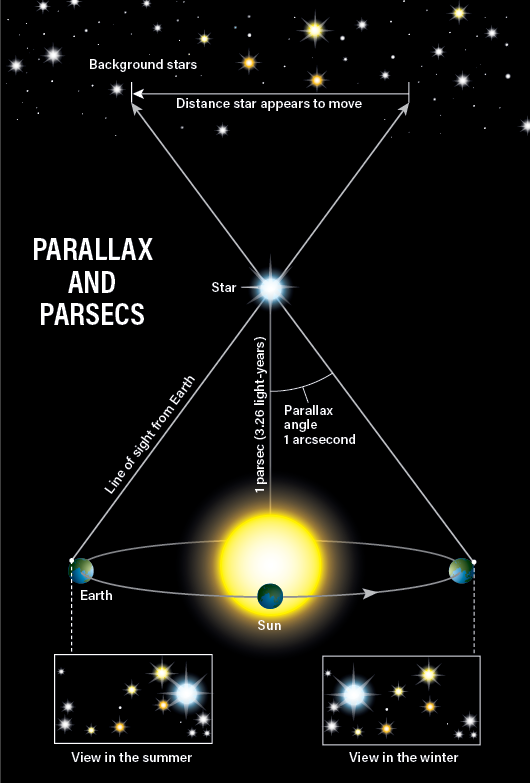
\includegraphics{img/parallax_parsecs.png}

}

\caption{Parallax and parsecs representation. Image readapted from:
https://www.astronomy.com/wp-content/uploads/sites/2/2023/02/parsec.png}

\end{figure}

\begin{itemize}
\item
  The parallax is generally measured in arcseconds (\emph{as}). 1
  arcsecond \(= \dfrac{1}{3600} \deg = \dfrac{1}{206,265}\) radians. You
  can show these conversions by recalling that
  \(1\ \rm{rad} = 57.3\deg = (57.3\times 60\times 60)\ \rm{as}=206,265\ \rm{as}\).
\item
  The parsec (\textbf{par}allax-\textbf{sec}ond, \emph{pc}) is defined
  as:
  \[ 1\ \rm{parsec} = \dfrac{1 au}{\rm{arcsecond\  in\  radians}} = 206,265\ au= \dfrac{648000}{\pi} \rm{au} \approx 3.086\times 10^{16}\rm{m}\].
\item
  A parallax of 1 arcsecond corresponds to a distance to the star of 1
  parsec (3.26 light-years).
\item
  Using trigonometry, the distance \(d\) to the star is given by:
\end{itemize}

\[
    d =\dfrac{1 \rm{au}}{\tan p}\simeq \dfrac{1}{p} \rm{au} 
\] \(\qquad\) where \(p\) is the parallax, and for this approximation we
used \(p\) measured in radians. Converting the parallax \(p\) to
\(p''\), from radians to arcseconds, we obtain the distance in parsec:
\[
    d \simeq\dfrac{206,265 \rm{au}}{p''}= \dfrac{1}{p''} \rm{pc} 
\]

\begin{Shaded}
\begin{Highlighting}[]
\ImportTok{import}\NormalTok{ warnings}
\NormalTok{warnings.filterwarnings(}\StringTok{\textquotesingle{}ignore\textquotesingle{}}\NormalTok{)}
\ImportTok{import}\NormalTok{ numpy }\ImportTok{as}\NormalTok{ np}
\ImportTok{import}\NormalTok{ math}
\NormalTok{AU }\OperatorTok{=} \DecValTok{149597870} \CommentTok{\# km}
\NormalTok{pc }\OperatorTok{=} \DecValTok{648000}\OperatorTok{/}\NormalTok{np.pi}\OperatorTok{*}\NormalTok{AU }\CommentTok{\# km}
\BuiltInTok{print}\NormalTok{(}\SpecialStringTok{f"1parsec = }\SpecialCharTok{\{}\NormalTok{pc}\SpecialCharTok{:1.3e\}}\SpecialStringTok{ km"}\NormalTok{)}
\end{Highlighting}
\end{Shaded}

\begin{verbatim}
1parsec = 3.086e+13 km
\end{verbatim}

\hypertarget{the-nearest-star-proxima-centauri}{%
\subsubsection{\texorpdfstring{3.4.2. \protect\hyperlink{toc0_}{The
nearest star: Proxima
Centauri}}{3.4.2. The nearest star: Proxima Centauri}}\label{the-nearest-star-proxima-centauri}}

The further a star is, the smaller the parallax angle.

The nearest star (Proxima Centauri) has a parallax of 0.7681 arcseconds.
This is \emph{very} tiny, but still, we are able to measure it! To give
you an idea of how small this is: - It is approximately the angle
subtended by an object having a diameter of 2 centimeters, positioned at
a distance of 5.3km! - The shift produced by the parallax against the
background would be \(1/2000^{th}\) the width of the Full Moon!

The parallax method is covered in the `Observational Methods' course, so
this is just a taster, but now knowing the parallax of Proxima Centauri
(or another star), we can find the distance to that.

\begin{Shaded}
\begin{Highlighting}[]
\CommentTok{\# The correct version}
\ImportTok{import}\NormalTok{ warnings}
\NormalTok{warnings.filterwarnings(}\StringTok{\textquotesingle{}ignore\textquotesingle{}}\NormalTok{)}
\ImportTok{import}\NormalTok{ math}
\ImportTok{import}\NormalTok{ numpy }\ImportTok{as}\NormalTok{ np}
\KeywordTok{def}\NormalTok{ arcsec\_to\_rad(p):}
\NormalTok{    rad }\OperatorTok{=}\NormalTok{ p}\OperatorTok{/}\DecValTok{206265}
    \ControlFlowTok{return}\NormalTok{ rad}

\NormalTok{p }\OperatorTok{=} \FloatTok{0.7681} \CommentTok{\# as}
\NormalTok{d\_pc }\OperatorTok{=} \DecValTok{1}\OperatorTok{/}\NormalTok{p }\CommentTok{\# pc}

\NormalTok{p\_rad }\OperatorTok{=}\NormalTok{ arcsec\_to\_rad(p)}
\NormalTok{d\_au }\OperatorTok{=} \DecValTok{1}\OperatorTok{/}\NormalTok{p\_rad }\CommentTok{\# au}
\NormalTok{d\_km }\OperatorTok{=}\NormalTok{ d\_au}\OperatorTok{*}\NormalTok{AU }\CommentTok{\# km}
\BuiltInTok{print}\NormalTok{(}\SpecialStringTok{f"p = }\SpecialCharTok{\{}\NormalTok{p}\SpecialCharTok{\}}\SpecialStringTok{ as"}\NormalTok{)}
\BuiltInTok{print}\NormalTok{(}\SpecialStringTok{f"d = 1/p pc = 1/}\SpecialCharTok{\{}\NormalTok{p}\SpecialCharTok{\}}\SpecialStringTok{ pc = }\SpecialCharTok{\{}\NormalTok{d\_pc}\SpecialCharTok{:1.1e\}}\SpecialStringTok{ pc"}\NormalTok{)}
\BuiltInTok{print}\NormalTok{(}\SpecialStringTok{f"d = 1/p au = 20625/p au = 20625/}\SpecialCharTok{\{}\NormalTok{p}\SpecialCharTok{\}}\SpecialStringTok{ au = }\SpecialCharTok{\{}\NormalTok{d\_au}\SpecialCharTok{:1.1e\}}\SpecialStringTok{ au"}\NormalTok{)}
\BuiltInTok{print}\NormalTok{(}\SpecialStringTok{f"d = }\SpecialCharTok{\{}\NormalTok{d\_au}\SpecialCharTok{:1.1e\}}\SpecialStringTok{ au * 149597870 km = }\SpecialCharTok{\{}\NormalTok{d\_km}\SpecialCharTok{:1.1e\}}\SpecialStringTok{ km"}\NormalTok{)}
\BuiltInTok{print}\NormalTok{(}\SpecialStringTok{f"The distance from Proxima Centauri is = }\SpecialCharTok{\{}\NormalTok{d\_pc}\SpecialCharTok{:1.1e\}}\SpecialStringTok{ pc = }\SpecialCharTok{\{}\NormalTok{d\_au}\SpecialCharTok{:1.1e\}}\SpecialStringTok{ au = }\SpecialCharTok{\{}\NormalTok{d\_km}\SpecialCharTok{:1.1e\}}\SpecialStringTok{ km"}\NormalTok{)}
\end{Highlighting}
\end{Shaded}

\begin{verbatim}
p = 0.7681 as
d = 1/p pc = 1/0.7681 pc = 1.3e+00 pc
d = 1/p au = 20625/p au = 20625/0.7681 au = 2.7e+05 au
d = 2.7e+05 au * 149597870 km = 4.0e+13 km
The distance from Proxima Centauri is = 1.3e+00 pc = 2.7e+05 au = 4.0e+13 km
\end{verbatim}

\hypertarget{spot-the-mistake-question}{%
\subsubsection{\texorpdfstring{3.4.3. \protect\hyperlink{toc0_}{`Spot
the mistake'
question:}}{3.4.3. `Spot the mistake' question:}}\label{spot-the-mistake-question}}

An unknown star has a parallax of 379.21 mas. Your messy lecturer tried
to calculate the distance to the star but she must have made some
mistakes because something looks wrong. Can you tell what?

\textbf{Hints}

\begin{itemize}
\tightlist
\item
  Hint 1: check the orders of magnitude, do they seem reasonable?
\item
  Hint 2: compare these orders of magnitude with the ones found for
  Proxima Centauri, any red flags?
\item
  Hint 3: the units are important!
\end{itemize}

\begin{Shaded}
\begin{Highlighting}[]
\CommentTok{\# This is the version with mistakes}
\ImportTok{import}\NormalTok{ math}

\NormalTok{p }\OperatorTok{=} \FloatTok{379.21}\OperatorTok{/}\DecValTok{10000} \CommentTok{\# as }
\NormalTok{d\_pc }\OperatorTok{=} \DecValTok{206265}\OperatorTok{/}\NormalTok{p }\CommentTok{\# pc}

\NormalTok{d\_au }\OperatorTok{=} \DecValTok{1}\OperatorTok{/}\NormalTok{p }\CommentTok{\# au}

\NormalTok{AU }\OperatorTok{=} \DecValTok{149597870} \CommentTok{\# km}
\NormalTok{d\_km }\OperatorTok{=}\NormalTok{ d\_au}\OperatorTok{*}\NormalTok{AU }\CommentTok{\# km}
\BuiltInTok{print}\NormalTok{(}\SpecialStringTok{f"The distance to the star is = }\SpecialCharTok{\{}\NormalTok{d\_pc}\SpecialCharTok{:1.1e\}}\SpecialStringTok{ pc = }\SpecialCharTok{\{}\NormalTok{d\_au}\SpecialCharTok{:1.1e\}}\SpecialStringTok{ au = }\SpecialCharTok{\{}\NormalTok{d\_km}\SpecialCharTok{:1.1e\}}\SpecialStringTok{ km? Something does not look right... find the mistakes!"}\NormalTok{)}
\end{Highlighting}
\end{Shaded}

The distance to the star is = 5.4e+06 pc = 2.6e+01 au = 3.9e+09 km?
Something does not look right\ldots{} find the mistakes!

\begin{Shaded}
\begin{Highlighting}[]
\CommentTok{\# The version with mistakes, where I made a wrong units conversion and I swapped the formulas for d in pc and in au}
\ImportTok{import}\NormalTok{ warnings}
\NormalTok{warnings.filterwarnings(}\StringTok{\textquotesingle{}ignore\textquotesingle{}}\NormalTok{)}
\ImportTok{import}\NormalTok{ math}

\NormalTok{p }\OperatorTok{=} \FloatTok{379.21}\OperatorTok{/}\DecValTok{10000} \CommentTok{\# as }
\NormalTok{d\_pc }\OperatorTok{=} \DecValTok{206265}\OperatorTok{/}\NormalTok{p }\CommentTok{\# pc}

\NormalTok{d\_au }\OperatorTok{=} \DecValTok{1}\OperatorTok{/}\NormalTok{p }\CommentTok{\# au}

\NormalTok{AU }\OperatorTok{=} \DecValTok{149597870} \CommentTok{\# km}
\NormalTok{d\_km }\OperatorTok{=}\NormalTok{ d\_au}\OperatorTok{*}\NormalTok{AU }\CommentTok{\# km}
\BuiltInTok{print}\NormalTok{(}\SpecialStringTok{f"The distance to the star is = }\SpecialCharTok{\{}\NormalTok{d\_pc}\SpecialCharTok{:1.1e\}}\SpecialStringTok{ pc = }\SpecialCharTok{\{}\NormalTok{d\_au}\SpecialCharTok{:1.1e\}}\SpecialStringTok{ au = }\SpecialCharTok{\{}\NormalTok{d\_km}\SpecialCharTok{:1.1e\}}\SpecialStringTok{ km? Something does not look right... find the mistakes!"}\NormalTok{)}
\end{Highlighting}
\end{Shaded}

\begin{verbatim}
The distance to the star is = 5.4e+06 pc = 2.6e+01 au = 3.9e+09 km? Something does not look right... find the mistakes!
\end{verbatim}

\textbf{Solution}

Below is the solution to the question. Something was clearly wrong with
the orders of magnitudes of the values obtained in the wrong solution: -
the distance in pc can not be larger than the distance in au! Those
orders of magnitude are clearly off! - if you compare this with the
values obtained for Proxima Centauri, you should expect approximately
the same orders of magnitude - \(10^6\) pc would be way too far to be
able to use the parallax method to measure the distance: the most
precise and reliable measurements of the parallax (with the Hubble Space
Telescope and Gaia space mission), can measure distances of the order of
\(10^3\rm{pc}\).

\begin{Shaded}
\begin{Highlighting}[]
\CommentTok{\# The correct version}
\ImportTok{import}\NormalTok{ warnings}
\NormalTok{warnings.filterwarnings(}\StringTok{\textquotesingle{}ignore\textquotesingle{}}\NormalTok{)}
\ImportTok{import}\NormalTok{ math}

\NormalTok{p }\OperatorTok{=} \FloatTok{379.21}\OperatorTok{/}\DecValTok{1000} \CommentTok{\# as \textless{}{-} the units conversion was wrong}
\NormalTok{d\_pc }\OperatorTok{=} \DecValTok{1}\OperatorTok{/}\NormalTok{p }\CommentTok{\# pc \textless{}{-} This formula for the distance in pc was swapped with the one below for the distance in au}

\NormalTok{d\_au }\OperatorTok{=} \DecValTok{206265}\OperatorTok{/}\NormalTok{p }\CommentTok{\# au \textless{}{-}}

\NormalTok{AU }\OperatorTok{=} \DecValTok{149597870} \CommentTok{\# km}
\NormalTok{d\_km }\OperatorTok{=}\NormalTok{ d\_au}\OperatorTok{*}\NormalTok{AU }\CommentTok{\# km}
\BuiltInTok{print}\NormalTok{(}\SpecialStringTok{f"The distance to the star is = }\SpecialCharTok{\{}\NormalTok{d\_pc}\SpecialCharTok{:1.1e\}}\SpecialStringTok{ pc = }\SpecialCharTok{\{}\NormalTok{d\_au}\SpecialCharTok{:1.1e\}}\SpecialStringTok{ au = }\SpecialCharTok{\{}\NormalTok{d\_km}\SpecialCharTok{:1.1e\}}\SpecialStringTok{ km}
\end{Highlighting}
\end{Shaded}

The distance to the star is = 2.6e+00 pc = 5.4e+05 au = 8.1e+13 km

\begin{Shaded}
\begin{Highlighting}[]
\CommentTok{\# The correct version}
\ImportTok{import}\NormalTok{ warnings}
\NormalTok{warnings.filterwarnings(}\StringTok{\textquotesingle{}ignore\textquotesingle{}}\NormalTok{)}
\ImportTok{import}\NormalTok{ math}

\NormalTok{p }\OperatorTok{=} \FloatTok{379.21}\OperatorTok{/}\DecValTok{1000} \CommentTok{\# as \textless{}{-} the units conversion was wrong}
\NormalTok{d\_pc }\OperatorTok{=} \DecValTok{1}\OperatorTok{/}\NormalTok{p }\CommentTok{\# pc \textless{}{-} This formula for the distance in pc was swapped with the one below for the distance in au}

\NormalTok{d\_au }\OperatorTok{=} \DecValTok{206265}\OperatorTok{/}\NormalTok{p }\CommentTok{\# au}

\NormalTok{AU }\OperatorTok{=} \DecValTok{149597870} \CommentTok{\# km}
\NormalTok{d\_km }\OperatorTok{=}\NormalTok{ d\_au}\OperatorTok{*}\NormalTok{AU }\CommentTok{\# km}
\BuiltInTok{print}\NormalTok{(}\SpecialStringTok{f"The distance to the star is = }\SpecialCharTok{\{}\NormalTok{d\_pc}\SpecialCharTok{:1.1e\}}\SpecialStringTok{ pc = }\SpecialCharTok{\{}\NormalTok{d\_au}\SpecialCharTok{:1.1e\}}\SpecialStringTok{ au = }\SpecialCharTok{\{}\NormalTok{d\_km}\SpecialCharTok{:1.1e\}}\SpecialStringTok{ km"}\NormalTok{)}
\end{Highlighting}
\end{Shaded}

\begin{verbatim}
The distance to the star is = 2.6e+00 pc = 5.4e+05 au = 8.1e+13 km
\end{verbatim}

\hypertarget{transit-method}{%
\subsection{\texorpdfstring{3.5. \protect\hyperlink{toc0_}{Transit
method}}{3.5. Transit method}}\label{transit-method}}

The parallax was also originally proposed as a way to determine the
distance to the Sun by the Scottish astronomer James Gregory, in 1663,
using the transit of Venus. Gregory is seldom given any credits for this
idea and usually all the credits goes to Edmund Halley for some reason
(can anyone find out why?).

In 1677, at the age of 20, Halley travelled to St Helena to map the
Southern Skies and observed a transit of Mercury on November 7th. Like
Gregory, he suggested that the transit of a planet like Venus could be
used as a method to measure the distance to the Sun, using parallax.

Here is the translation of Halley's publication about this idea:
https://eclipse.gsfc.nasa.gov/transit/HalleyParallax.html

\begin{figure}

{\centering 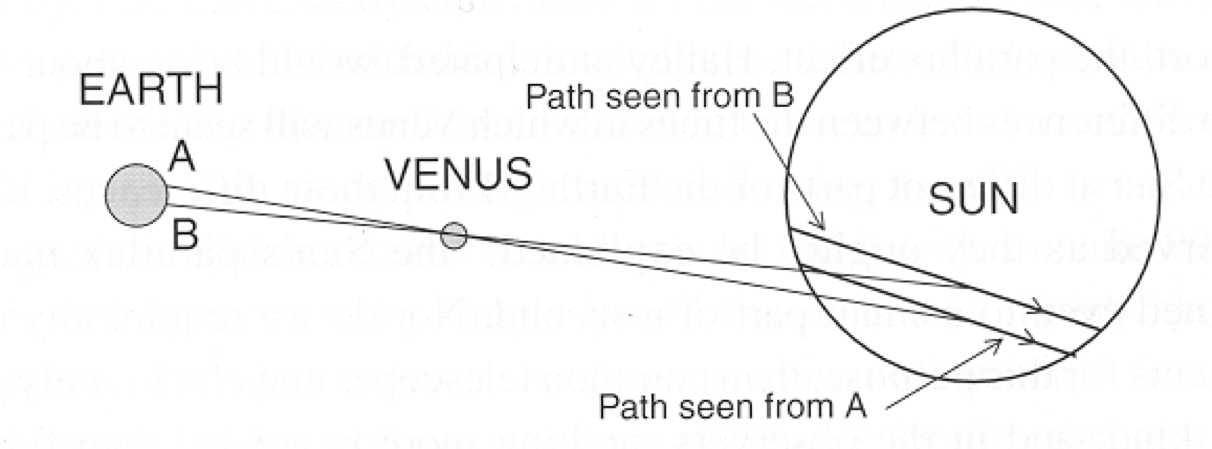
\includegraphics{img/TransitMethod.png}

}

\caption{Transit Method}

\end{figure}

According to `Halley's method', two observers (A and B in the figure
above) have to be positioned at a great distance from each other, but
both located on the side of Earth facing the Sun at the time of the
transit. Each observer would precisely measure the times that Venus
appear to be in different positions (contact points) relative to the
Sun. The observers would see different chords of the planet's trajectory
across the disk of the sun due to parallax. Venus forms two similar
triangles with the Earth and the Sun at their opposite edges. Since the
triangles are similar, the projected distance on the Sun can be found by
comparing it to a known baseline on Earth. Once the angle shift is
measured, the distances to Venus and then to the Sun can be determined
using trigonometry.

Modern techniques use radar echo ranging to measure distances in the
Solar System very precisely.

\hypertarget{how-big-are-stars}{%
\section{\texorpdfstring{4. \protect\hyperlink{toc0_}{How big are
stars?}}{4. How big are stars?}}\label{how-big-are-stars}}

\hypertarget{how-big-is-the-sun}{%
\subsection{\texorpdfstring{4.1. \protect\hyperlink{toc0_}{How big is
the Sun?}}{4.1. How big is the Sun?}}\label{how-big-is-the-sun}}

We can deduce the width of the sun if we know its angular diameter
\(\alpha\) and the distance \(D\).

For small angles, \(\alpha \approx \frac{2R_\odot}{D}\).

WARNING: This formula uses \emph{radians} for \(\alpha\)

Since the Sun's angular diameter is
\(\alpha\approx 0.5^\circ \approx 32 \ \rm{arcmin} \approx 9.3\times 10^{-3} \rm{rad}\),
and we know its distance (from Earth)
\(D = 1 \rm{au} = 149,597,870 \ \rm{km}\), we can now calculate the size
of the Sun.

\begin{Shaded}
\begin{Highlighting}[]
\ImportTok{import}\NormalTok{ warnings}
\NormalTok{warnings.filterwarnings(}\StringTok{\textquotesingle{}ignore\textquotesingle{}}\NormalTok{)}
\ImportTok{import}\NormalTok{ math}
\NormalTok{AU }\OperatorTok{=} \DecValTok{149597870} \CommentTok{\# km}
\NormalTok{ang\_diameter\_arcm }\OperatorTok{=} \DecValTok{32} \CommentTok{\# angular diameter of Sun is about 32 minutes of arc}
\NormalTok{ang\_diameter }\OperatorTok{=}\NormalTok{ ang\_diameter\_arcm}\OperatorTok{/}\DecValTok{60} \OperatorTok{*}\NormalTok{ math.pi}\OperatorTok{/}\DecValTok{180} 
\CommentTok{\# ang\_diameter = ang\_diameter\_rad}
\NormalTok{diameter }\OperatorTok{=}\NormalTok{ AU }\OperatorTok{*}\NormalTok{ ang\_diameter}
\BuiltInTok{print}\NormalTok{(}\SpecialStringTok{f"1 au = }\SpecialCharTok{\{}\NormalTok{AU}\SpecialCharTok{:1.3e\}}\SpecialStringTok{ km"}\NormalTok{)}
\BuiltInTok{print}\NormalTok{(}\SpecialStringTok{f"angular diameter of the sun =  }\SpecialCharTok{\{}\NormalTok{ang\_diameter}\SpecialCharTok{:.3e\}}\SpecialStringTok{ radians"}\NormalTok{)}
\BuiltInTok{print}\NormalTok{(}\SpecialStringTok{f"Diameter of Sun = }\SpecialCharTok{\{}\NormalTok{diameter}\SpecialCharTok{:.0f\}}\SpecialStringTok{ km"}\NormalTok{)}
\BuiltInTok{print}\NormalTok{(}\SpecialStringTok{f"Radius of Sun = }\SpecialCharTok{\{}\NormalTok{diameter}\OperatorTok{/}\DecValTok{2}\SpecialCharTok{:.0f\}}\SpecialStringTok{ km"}\NormalTok{)}
\end{Highlighting}
\end{Shaded}

\begin{verbatim}
1 au = 1.496e+08 km
angular diameter of the sun =  9.308e-03 radians
Diameter of Sun = 1392520 km
Radius of Sun = 696260 km
\end{verbatim}

The accepted radius is \(6.957\times 10^5\) km.

\hypertarget{what-about-other-stars}{%
\subsection{\texorpdfstring{4.2. \protect\hyperlink{toc0_}{What about
other
stars?}}{4.2. What about other stars?}}\label{what-about-other-stars}}

Here is a video showing a comparison between star sizes:
https://www.youtube.com/watch?v=HEheh1BH34Q

\hypertarget{a-comparison-of-some-star-sizes}{%
\subsubsection{\texorpdfstring{4.2.1. \protect\hyperlink{toc0_}{A
comparison of some star
sizes}}{4.2.1. A comparison of some star sizes}}\label{a-comparison-of-some-star-sizes}}

Here is a list of some selected examples of star radii, compared to the
Sun. Some stars, such as Sirius B, are much smaller than the Sun. (The
picture below shows an artistic impression of Sirius A and Sirius B.)

The typical range of star radii is roughly
\(10^{-3}R_\odot < R < 10^3 R_\odot\).

\begin{longtable}[]{@{}ll@{}}
\toprule\noalign{}
Name & Radius \\
\midrule\noalign{}
\endhead
\bottomrule\noalign{}
\endlastfoot
Sirius B & 0.008 \(R_\odot\) \\
Sirius A & 1.71 \(R_\odot\) \\
Arcturus & 12 \(R_\odot\) \\
Aldebaran & 22 \(R_\odot\) \\
Rigel & 78.9 \(R_\odot\) \\
Mira & 210 \(R_\odot\) \\
Betelgeuse & 320 \(R_\odot\) \\
\end{longtable}

\begin{figure}

{\centering 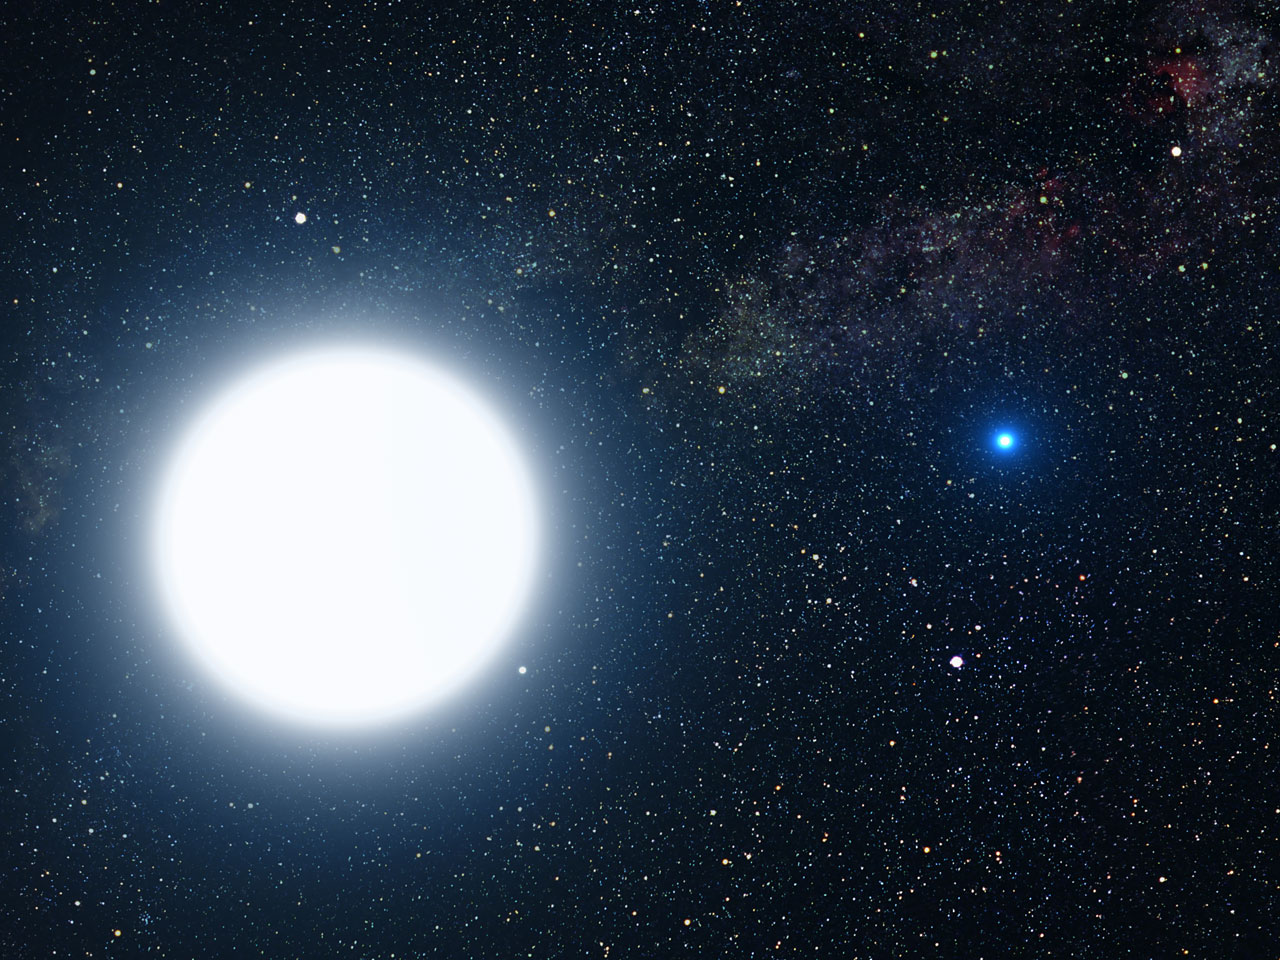
\includegraphics{img/siriusAB.jpeg}

}

\caption{Artistic impression of Sirius A (large blue-white star on the
left) and Sirius B (small blue white-dwarf star on the right)}

\end{figure}

\emph{Image credit: NASA, ESA and G. Bacon (STScI)}

\begin{itemize}
\tightlist
\item
  Sirius B is a very small but very hot white dwarf. It is even smaller
  than Earth, and it cannot be observed by the naked eye. Its companion
  star Sirius A, in contrast, is the brightest star in the sky
\item
  Betelgeuse -- at a distance of 650 l.y. is a red supergiant and rather
  short-lived star, the second brightest in Orion and the ninth
  brightest in the sky
\item
  It's close to the end of its life and en-route to a rather spectacular
  death within a million years or so
\item
  For Betelgeuse, the angular diameter \(\alpha\) is about 0.000014
  degrees (\(1.4\times 10^{-5}\) degrees)
\item
  Most stars have a much smaller angular diameter and cannot be directly
  imaged
\item
  We have to deduce their size indirectly! (more on this later)
\end{itemize}

\begin{figure}

{\centering 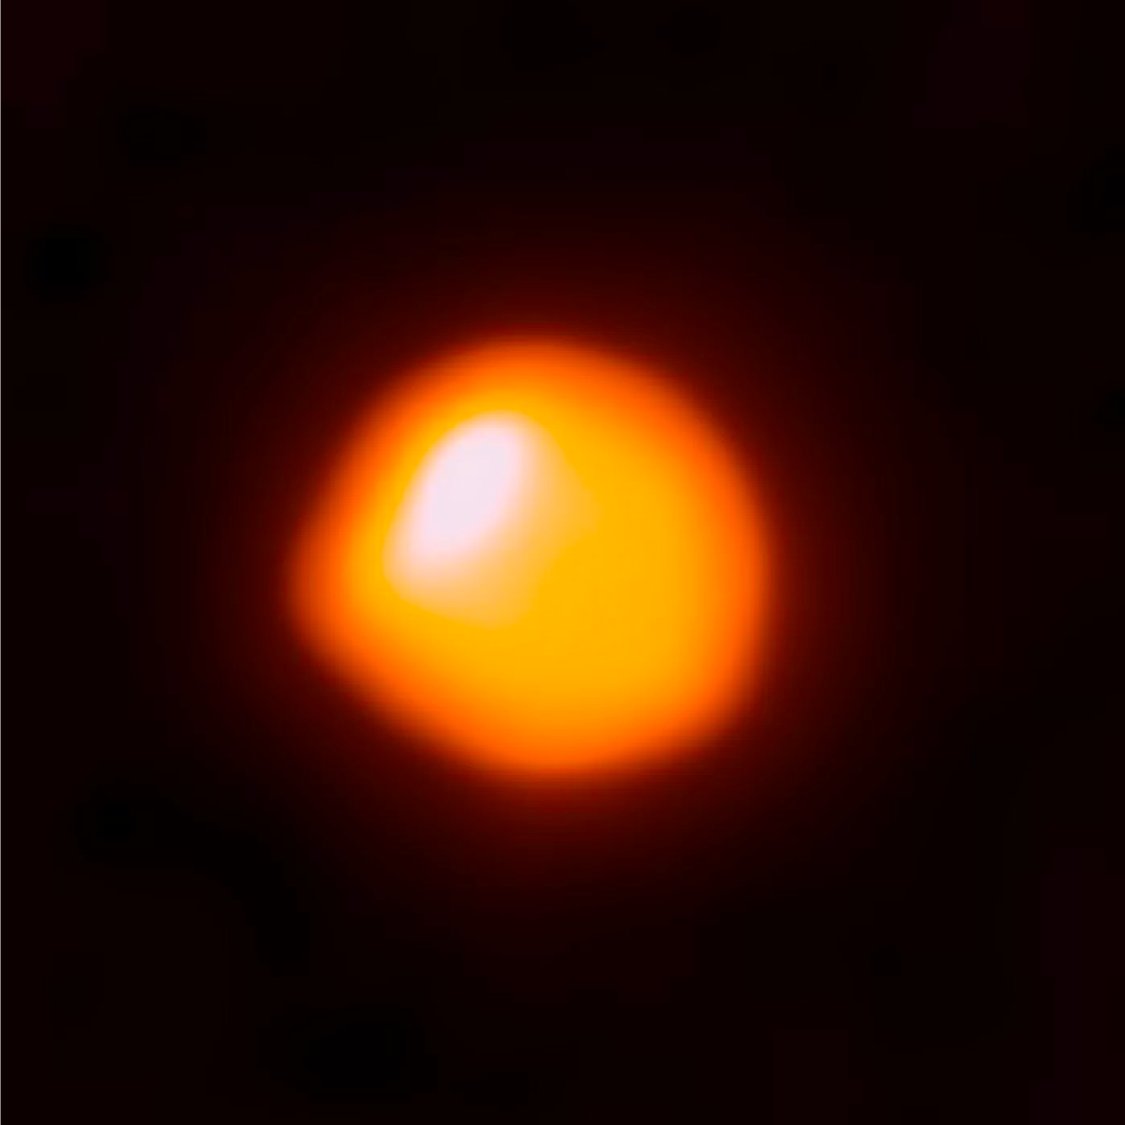
\includegraphics{img/Betelgeuse.png}

}

\caption{Betelgeuse}

\end{figure}

\emph{Image credit: ALMA (ESO/NAOJ/NRAO)/E. O'Gorman/P. Kervella}

\hypertarget{a-handy-guide-to-estimating-angular-diameters}{%
\subsection{\texorpdfstring{4.3. \protect\hyperlink{toc0_}{A handy guide
to estimating angular
diameters}}{4.3. A handy guide to estimating angular diameters}}\label{a-handy-guide-to-estimating-angular-diameters}}

You can estimate angular diameters using your hand! Extend your arm,
place the hand at a right angle and follow the intstructions of the
following figure to estimate different angles. This may not be useful to
determine the size of objects that are very far and appear too small,
such as stars, but can be useful to measure the angular distance between
two stars.

\begin{figure}

{\centering 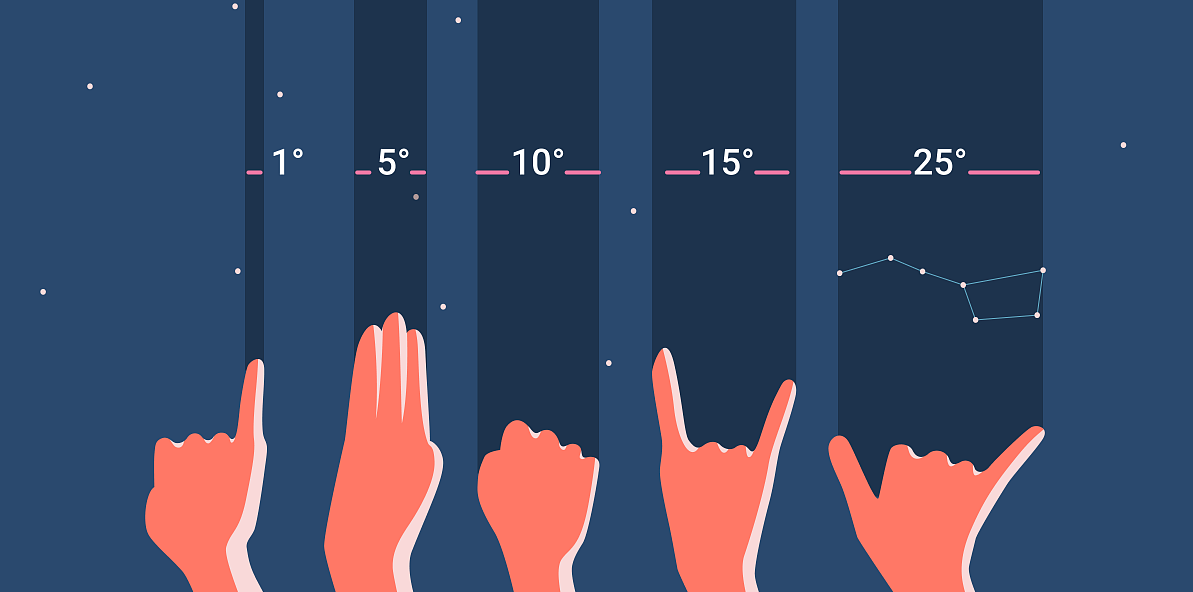
\includegraphics{img/measuring-sky-with-hand.png}

}

\caption{How to use hands to measure angular distances in the sky}

\end{figure}

\hypertarget{how-far-apart-are-the-stars}{%
\subsection{\texorpdfstring{4.4. \protect\hyperlink{toc0_}{How far apart
are the
stars?}}{4.4. How far apart are the stars?}}\label{how-far-apart-are-the-stars}}

Let's have a look at some orders of magnitude (this is a good resource
if you want to visualise them: https://scaleofuniverse.com/en-gb).

\begin{itemize}
\tightlist
\item
  The nearest star (Proxima Centauri) is about \(10^{16}\) m away.
\item
  Diameter of the Sun \textasciitilde{} \(10^{9}\) m.
\item
  The difference in scale is \(10^7\)m in distance, or
  \(10^{21}\)m\(^3\) in volume.
\item
  Relative to their size, stars are the most isolated structures in the
  universe.
\item
  If stars were grains of sand (\textasciitilde1 mm), they would be
  \textasciitilde10 km apart!
\item
  However, we find them in clusters and binaries - what explains this?
  (more on this later)
\end{itemize}

\hypertarget{how-bright-are-stars}{%
\section{\texorpdfstring{5. \protect\hyperlink{toc0_}{How bright are
stars?}}{5. How bright are stars?}}\label{how-bright-are-stars}}

If we try to answer this question based on our observations, we have to
keep in mind that the apparent brightness of a light source will vary
depending on its distance from the observer. The brightenss we observe
is therefore not an \emph{intrinsic} property of the stars, as it
depends on the distance between the observer and the stars.

This is the reason why we need to differentiate between the
\emph{apparent brightness} of a star and its \emph{luminosity}.

\hypertarget{apparent-brightness-and-luminosity}{%
\subsection{\texorpdfstring{5.1. \protect\hyperlink{toc0_}{Apparent
brightness and
luminosity}}{5.1. Apparent brightness and luminosity}}\label{apparent-brightness-and-luminosity}}

The \textbf{apparent brightness}, \(F\) (units {[}\(\rm{W/m}^2\){]}),
also referred to as the \emph{radiant flux} or \emph{power flux}, is the
total amount of energy emitted by a star, per unit time, crossing an
unit area. It is \emph{not} an intrinsic property of a star, because it
depends on the distance from the star.

The following figure can give you a better understanding of that. Each
square represents an unit area. The lightbulb, like a star, radiates
equally in every direction (i.e.~isotropically). The `rays' coming out
of the light source represent the flux. The farther the position of the
observer is from the source, the less flux the observer, in one unit
area, will receive. The relationship between the power flux, \(F\), and
the distance to the source, \(r\), is given by the inverse square law:
\[F\propto \dfrac{1}{r^2}.\] Since the light source radiates
isotropically (even though the figure below shows only a portion of the
rays), the power flux \(F\) is equal across all parts of the sphere.

\begin{figure}

{\centering 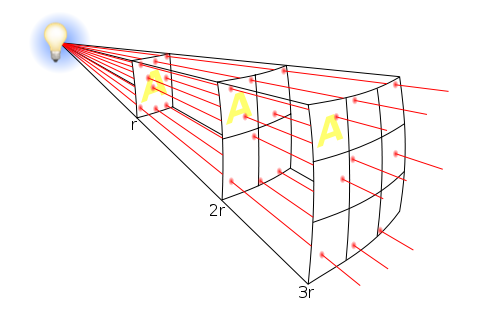
\includegraphics{img/inverse_square_law.png}

}

\caption{Inverse square law of the radiant flux of a light source}

\end{figure}

The \textbf{Luminosity} of a star, \(L\), measured in Watts (W) or
equivalently Joules per second (J/s), is its energy output per unit
time. The luminosity is the \emph{total} energy radiated in all the
directions in an unit time and it does not depend on the distance from
the observer: it is an intrinsic property of the star.

How are these two quantities related?

Imagine a sphere of radius \(r\) centered on a star, which is
isotropically radiating. Since the power flux \(F\) is equal across all
parts of the sphere and is the energy output, per unit time, crossing an
unit area, we need to divide the luminosity equally over the area of the
sphere, \(4\pi r^2\). Therefore \begin{equation}
F = \frac{L}{4\pi r^2}
\end{equation}

The apparent brightness depends on the luminosity and on the distance of
the observer from the star. From the formula above, you can see how two
stars of equal luminosity, located at different distances from Earth,
would have different apparent brightness.

\emph{Photometry} is the measurement of the quantity of light from a
star, i.e.~the flux of energy per unit time, per unit area, that we
receive at Earth.

For a particular star, if we know the luminosity (\(L\)) of the star and
its distance from Earth (\(r\)) we can calculate the flux using the
equation above.

\hypertarget{the-suns-luminosity}{%
\subsubsection{\texorpdfstring{5.1.1. \protect\hyperlink{toc0_}{The
Sun's
luminosity}}{5.1.1. The Sun's luminosity}}\label{the-suns-luminosity}}

For our Sun, we have:

\(F_\odot = 1361\, \mathrm{W/m^2}\) (The ``Solar Constant'', or ``Solar
irradiance'', sometimes indicated with the symbol \(S_\odot\) in
textbooks)

\(r = 1\, \mathrm{a.u.} \approx 1.5\times 10^{11}\, \mathrm{m}\)

so

\(L_\odot = 4\pi r^2 F = 3.8275 \times 10^{26}\, \mathrm{W}\)

\begin{Shaded}
\begin{Highlighting}[]
\ImportTok{import}\NormalTok{ scipy}
\ImportTok{from}\NormalTok{ scipy.constants }\ImportTok{import}\NormalTok{ pi, au, parsec}

\NormalTok{F }\OperatorTok{=} \FloatTok{1361.0} \CommentTok{\# W/m/m}
\NormalTok{r }\OperatorTok{=}\NormalTok{ au }\CommentTok{\# m}
\NormalTok{L }\OperatorTok{=}\NormalTok{ F}\OperatorTok{*}\DecValTok{4}\OperatorTok{*}\NormalTok{pi}\OperatorTok{*}\NormalTok{r}\OperatorTok{**}\DecValTok{2}

\BuiltInTok{print}\NormalTok{(}\SpecialStringTok{f\textquotesingle{}Power flux: F = }\SpecialCharTok{\{}\NormalTok{F}\SpecialCharTok{\}}\SpecialStringTok{ W/m/m\textquotesingle{}}\NormalTok{)}
\BuiltInTok{print}\NormalTok{(}\SpecialStringTok{f\textquotesingle{}r = 1au = }\SpecialCharTok{\{}\NormalTok{r}\SpecialCharTok{:1.4e\}}\SpecialStringTok{ m\textquotesingle{}}\NormalTok{)}
\BuiltInTok{print}\NormalTok{(}\SpecialStringTok{f\textquotesingle{}Luminosity: L =  F*4*pi*r**2 = }\SpecialCharTok{\{}\NormalTok{L}\SpecialCharTok{:1.4e\}}\SpecialStringTok{ W\textquotesingle{}}\NormalTok{)}
\end{Highlighting}
\end{Shaded}

\begin{verbatim}
Power flux: F = 1361.0 W/m/m
r = 1au = 1.4960e+11 m
Luminosity: L =  F*4*pi*r**2 = 3.8275e+26 W
\end{verbatim}

For other stars there is a large range of luminosities:

\(10^{-4}\,L_\odot < L < 10^{6}\,L_\odot\)

If we think of the least luminous star as a 100W incandescent lightbulb,
this huge range tells us that the most luminous star would be like the
entire world's power output

Future question: \textbf{Why is there this very large range?}

\hypertarget{spot-the-mistake-question-1}{%
\subsubsection{\texorpdfstring{5.1.2. \protect\hyperlink{toc0_}{`Spot
the mistake'
question}}{5.1.2. `Spot the mistake' question}}\label{spot-the-mistake-question-1}}

\textbf{What would the apparent brightness be for a star like the Sun at
a distance of 10 pc?} Something does not seem to make sense in the
answer below, why?

\begin{Shaded}
\begin{Highlighting}[]
\CommentTok{\# This is the version containing a mistake}
\NormalTok{L }\OperatorTok{=} \FloatTok{3.8275E26} \CommentTok{\# W}
\NormalTok{r }\OperatorTok{=} \DecValTok{10} \CommentTok{\#pc}
\NormalTok{F }\OperatorTok{=}\NormalTok{ L}\OperatorTok{/}\NormalTok{(}\DecValTok{4}\OperatorTok{*}\NormalTok{pi}\OperatorTok{*}\NormalTok{r}\OperatorTok{**}\DecValTok{2}\NormalTok{)}
\BuiltInTok{print}\NormalTok{(}\SpecialStringTok{f\textquotesingle{}Solar luminosity = }\SpecialCharTok{\{}\NormalTok{L}\SpecialCharTok{\}}\SpecialStringTok{ W\textquotesingle{}}\NormalTok{)}
\BuiltInTok{print}\NormalTok{(}\SpecialStringTok{f\textquotesingle{}Distance r = }\SpecialCharTok{\{}\NormalTok{r}\SpecialCharTok{\}}\SpecialStringTok{ pc\textquotesingle{}}\NormalTok{)}
\BuiltInTok{print}\NormalTok{(}\SpecialStringTok{f\textquotesingle{}Apparent brightness of the Sun at 10 parsec: F = }\SpecialCharTok{\{}\NormalTok{F}\SpecialCharTok{:1.4e\}}\SpecialStringTok{ W/m/m\textquotesingle{}}\NormalTok{)}
\end{Highlighting}
\end{Shaded}

\begin{verbatim}
Solar luminosity = 3.8275e+26 W
Distance r = 10 pc
Apparent brightness of the Sun at 10 parsec: F = 3.0458e+23 W/m/m
\end{verbatim}

\begin{Shaded}
\begin{Highlighting}[]
\CommentTok{\# This is the version containing a mistake}
\NormalTok{L }\OperatorTok{=} \FloatTok{3.8275E26} \CommentTok{\# W}
\NormalTok{r }\OperatorTok{=} \DecValTok{10} \CommentTok{\#pc}
\NormalTok{F }\OperatorTok{=}\NormalTok{ L}\OperatorTok{/}\NormalTok{(}\DecValTok{4}\OperatorTok{*}\NormalTok{pi}\OperatorTok{*}\NormalTok{r}\OperatorTok{**}\DecValTok{2}\NormalTok{)}
\BuiltInTok{print}\NormalTok{(}\SpecialStringTok{f\textquotesingle{}Solar luminosity = }\SpecialCharTok{\{}\NormalTok{L}\SpecialCharTok{\}}\SpecialStringTok{ W\textquotesingle{}}\NormalTok{)}
\BuiltInTok{print}\NormalTok{(}\SpecialStringTok{f\textquotesingle{}Distance r = }\SpecialCharTok{\{}\NormalTok{r}\SpecialCharTok{\}}\SpecialStringTok{ pc\textquotesingle{}}\NormalTok{)}
\BuiltInTok{print}\NormalTok{(}\SpecialStringTok{f\textquotesingle{}Apparent brightness of the Sun at 10 parsec: F = }\SpecialCharTok{\{}\NormalTok{F}\SpecialCharTok{\}}\SpecialStringTok{ W/m/m\textquotesingle{}}\NormalTok{)}

\NormalTok{Solar luminosity }\OperatorTok{=} \FloatTok{3.8275e+26}\NormalTok{ W}
\NormalTok{Distance r }\OperatorTok{=} \DecValTok{10}\NormalTok{ pc}
\NormalTok{Apparent brightness of the Sun at }\DecValTok{10}\NormalTok{ parsec: F }\OperatorTok{=} \FloatTok{3.0458e+23}\NormalTok{ W}\OperatorTok{/}\NormalTok{m}\OperatorTok{/}\NormalTok{m}
\end{Highlighting}
\end{Shaded}

Does this make sense?

\textbf{Hints}

Hint 1: compare this apparent brightness obtained below with the value
of the power flux used (the Solar constant) in the previous example.
What is wrong?

Hint 2: Do a `sanity check' of the units in the quantities used above.
Does it seem correct?

If we compare this value obtained for the apparent brightness,
\(F=3.046\times 10^{23} \mathrm{W/m}^2\), with the Solar constant used
in the previous example, \(F_\odot = 1361 \mathrm{W/m}^2\), we can
immediately notice that something is wrong. If we are observing the Sun
from a further position of 10pc instead of 1au, we cannot expect it to
appear brighter!

Let's do a dimensional analysis `sanity check' by writing down the units
of the quantities given above, and by replacing them in the formula to
determine the flux from the luminosity:
\[ F=\frac{L}{4\pi r^2} \implies [W/m^2] = \frac{[W]}{[pc]^2} \] This
does not return an identity since \([m]\neq [pc]\), so now we know where
made a mistake, by just checking the units! To calculate the value of
the flux correctly, you need to convert the distance from parsecs to
meters, because the flux should be written in units of {[}\(W/m^2\){]}!

\begin{Shaded}
\begin{Highlighting}[]
\CommentTok{\# Correct version}
\ImportTok{import}\NormalTok{ scipy}
\ImportTok{from}\NormalTok{ scipy.constants }\ImportTok{import}\NormalTok{ pi, parsec}

\NormalTok{L }\OperatorTok{=} \FloatTok{3.8275E26} \CommentTok{\# W}
\NormalTok{r }\OperatorTok{=} \DecValTok{10}\OperatorTok{*}\NormalTok{parsec }\CommentTok{\#pc}
\NormalTok{F }\OperatorTok{=}\NormalTok{ L}\OperatorTok{/}\NormalTok{(}\DecValTok{4}\OperatorTok{*}\NormalTok{pi}\OperatorTok{*}\NormalTok{r}\OperatorTok{**}\DecValTok{2}\NormalTok{)}
\BuiltInTok{print}\NormalTok{(}\SpecialStringTok{f\textquotesingle{}Solar luminosity = }\SpecialCharTok{\{}\NormalTok{L}\SpecialCharTok{\}}\SpecialStringTok{ W\textquotesingle{}}\NormalTok{)}
\BuiltInTok{print}\NormalTok{(}\SpecialStringTok{f\textquotesingle{}Distance r = 10 pc = }\SpecialCharTok{\{}\NormalTok{r}\SpecialCharTok{:1.4e\}}\SpecialStringTok{ m\textquotesingle{}}\NormalTok{)}
\BuiltInTok{print}\NormalTok{(}\SpecialStringTok{f\textquotesingle{}Apparent brightness of the Sun at 10 parsec: F = }\SpecialCharTok{\{}\NormalTok{F}\SpecialCharTok{:1.4e\}}\SpecialStringTok{ W/m/m\textquotesingle{}}\NormalTok{)}

\NormalTok{Solar luminosity }\OperatorTok{=} \FloatTok{3.8275e+26}\NormalTok{ W}
\NormalTok{Distance r }\OperatorTok{=} \DecValTok{10}\NormalTok{ pc }\OperatorTok{=} \FloatTok{3.0857e+17}\NormalTok{ m}
\NormalTok{Apparent brightness of the Sun at }\DecValTok{10}\NormalTok{ parsec: F }\OperatorTok{=} \FloatTok{3.1989e{-}10}\NormalTok{ W}\OperatorTok{/}\NormalTok{m}\OperatorTok{/}\NormalTok{m}
\end{Highlighting}
\end{Shaded}

\begin{Shaded}
\begin{Highlighting}[]
\CommentTok{\# Correct version}
\ImportTok{import}\NormalTok{ scipy}
\ImportTok{from}\NormalTok{ scipy.constants }\ImportTok{import}\NormalTok{ pi, parsec}

\NormalTok{L }\OperatorTok{=} \FloatTok{3.8275E26} \CommentTok{\# W}
\NormalTok{r }\OperatorTok{=} \DecValTok{10}\OperatorTok{*}\NormalTok{parsec }\CommentTok{\#pc}
\NormalTok{F }\OperatorTok{=}\NormalTok{ L}\OperatorTok{/}\NormalTok{(}\DecValTok{4}\OperatorTok{*}\NormalTok{pi}\OperatorTok{*}\NormalTok{r}\OperatorTok{**}\DecValTok{2}\NormalTok{)}
\BuiltInTok{print}\NormalTok{(}\SpecialStringTok{f\textquotesingle{}Solar luminosity = }\SpecialCharTok{\{}\NormalTok{L}\SpecialCharTok{\}}\SpecialStringTok{ W\textquotesingle{}}\NormalTok{)}
\BuiltInTok{print}\NormalTok{(}\SpecialStringTok{f\textquotesingle{}Distance r = 10 pc = }\SpecialCharTok{\{}\NormalTok{r}\SpecialCharTok{:1.4e\}}\SpecialStringTok{ m\textquotesingle{}}\NormalTok{)}
\BuiltInTok{print}\NormalTok{(}\SpecialStringTok{f\textquotesingle{}Apparent brightness of the Sun at 10 parsec: F = }\SpecialCharTok{\{}\NormalTok{F}\SpecialCharTok{:1.4e\}}\SpecialStringTok{ W/m/m\textquotesingle{}}\NormalTok{)}
\end{Highlighting}
\end{Shaded}

\begin{verbatim}
Solar luminosity = 3.8275e+26 W
Distance r = 10 pc = 3.0857e+17 m
Apparent brightness of the Sun at 10 parsec: F = 3.1989e-10 W/m/m
\end{verbatim}

\textbf{Sanity checks}

Get the habit of doing `sanity checks' of the dimensional analysis and
units when you use or derive formulas. This will help you spot some
mistakes quickly and is incredibly useful to rederive some formulas
sometime. In the formula above for instance, we know that the apparent
brightness \(F\) has units of {[}W/m \(^2\){]} and that the luminosity
\(L\) has units of {[}W{]}. Writing the units of each side of Equation
(1) we see that: \$ {[}W/m\^{}2{]}=\dfrac{[W]}{[m^2]}\$, which as
expected satisfies the identity, meaning that the formula is
dimensionally correct.

\hypertarget{stellar-magnitude-scales}{%
\subsection{\texorpdfstring{5.2. \protect\hyperlink{toc0_}{Stellar
magnitude
scales}}{5.2. Stellar magnitude scales}}\label{stellar-magnitude-scales}}

The flux from even nearby stars is tiny, but many bright stars are
distinguished by the naked eye. The human eye (like hearing) responds
logarithmically to stimulus. When comparing the flux densities of three
stars in a 1:10:100 ratio, the perceived brightness gap between the
first and second star appears to be the same as the difference between
the second and third star. This equality in perceived brightness gaps
illustrates that human perception of brightness operates on a
logarithmic scale. Therefore, before modern photometry, astronomers had
a scale based on their own naked-eye observations: \textbf{stellar
(apparent) magnitude}.

\hypertarget{apparent-magnitude}{%
\subsubsection{\texorpdfstring{5.2.1. \protect\hyperlink{toc0_}{Apparent
magnitude}}{5.2.1. Apparent magnitude}}\label{apparent-magnitude}}

This system to measure the stars brightness was first introduced by the
Greek astronomer Hipparchos, who compiled a catalog of 850 stars with
their positions and their \emph{apparent magnitudes} on a scale from
\(m=1\), being the brightest stars, to \(m=6\), being the faintest
stars. The apparent magnitude depends on the position of the observer
the same way as the flux does (in fact, we will see in the following how
these two quantities are related).

The image below shows an example of a star catalog created by ancient
Greek astronomers.

\begin{figure}

{\centering 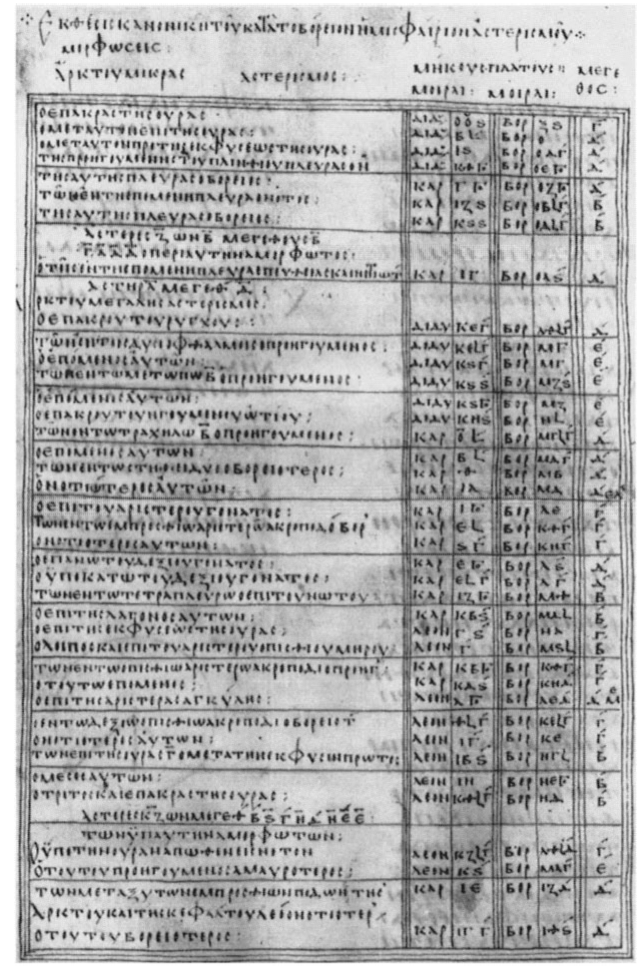
\includegraphics{img/Almagest.png}

}

\caption{Almagest}

\end{figure}

\emph{Almagest} Ptolemy, c.~150AD image credit: Bibliothèque Nationale,
Paris

The English translation reads

\begin{figure}

{\centering 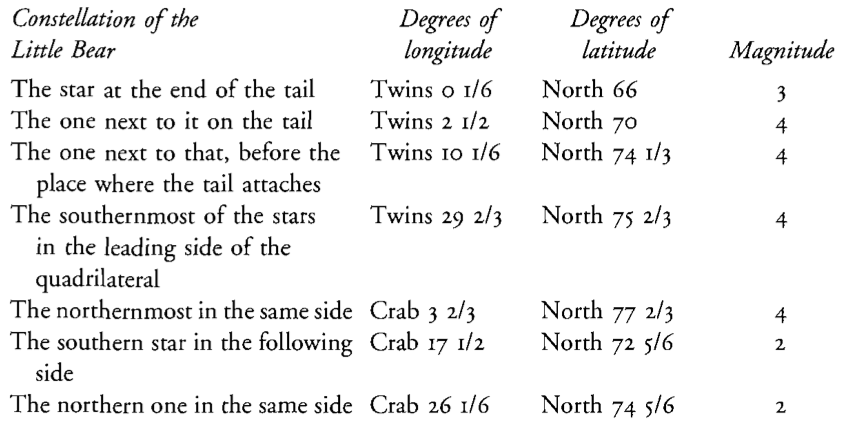
\includegraphics{img/AlmagestTranslation.png}

}

\caption{Almagest translated}

\end{figure}

We can still recognise the constellations and find these stars today!

The modern names and magnitudes for these stars are

\begin{longtable}[]{@{}ll@{}}
\toprule\noalign{}
Modern Name & Magnitude \\
\midrule\noalign{}
\endhead
\bottomrule\noalign{}
\endlastfoot
Polaris & 1.98 \\
Yildun & 4.35 \\
\(\epsilon\) Umi & 4.21 \\
Alasco & 4.95 \\
Ahfa al Farkadain & 4.29 \\
Pherkad & 3.04 \\
Kochab & 2.07 \\
\end{longtable}

Image credit: By IAU and Sky \& Telescope magazine (Roger Sinnott \&
Rick Fienberg) - {[}1{]}, CC BY 3.0, Link

Note that some of the magnitudes of the little bear stars have changed
since ancient times. Partly this is because the scientific definition
and measurements are more precise, but also Polaris is a variable star
(its brightness changes).

The apparent magnitude scale introduced by Hipparchos has been replaced
by Pogson in 1856 and is no longer limited to values between 1 and 6, it
now extends between m=-26.83 for the Sun to over m=30 for the faintest
object, but the new classification kept these characteristics:

\begin{itemize}
\tightlist
\item
  5 magnitude steps correspond to a factor of 100 in apparent brightness
\item
  A difference of 1 magnitude corresponds to an apparent brightness
  ratio of \(100^{1/5}\simeq 2.512\),
  i.e.~\(\dfrac{F_{m+1}}{F_m}=100^{1/5}\)
\item
  Lower magnitudes are \emph{brighter}
\item
  The zero point of the apparent magnitude has been
  \emph{conventionally} determined
\end{itemize}

The \emph{apparent magnitude} \(m\) is a measure of a star's apparent
brightness, i.e.~the flux received from the star, and it therefore
depends on how close the star is to the observer.

The definition of the apparent magnitude is based on the difference
between magnitudes and corresponds to the ratio between two stars'
fluxes, as stated in the properties above.

If we consider two stars with measured fluxes (units \(W/m^2\)) \(F_1\)
and \(F_2\), their apparent magnitudes will be related by

\begin{align}
m_1 - m_2 = -2.5 \log_{10} \frac{F_1}{F_2}
\end{align}

\hypertarget{apparent-magnitude-zero-point-convention}{%
\paragraph{\texorpdfstring{5.2.1.1. \protect\hyperlink{toc0_}{Apparent
magnitude zero point
convention}}{5.2.1.1. Apparent magnitude zero point convention}}\label{apparent-magnitude-zero-point-convention}}

The values of the apparent magnitudes are determined in relation to a
zero point value \(m=0\). By convention, this corresponds to an observed
flux of \(F_0 = 2.518 × 10^{−8} \ \mathrm{W m}^{−2}\). (Reference: IAU
2015 resolution)

The apparent magnitude of a star is therefore conventionally defined as

\begin{align}
m = -2.5 \log_{10}{\frac{F}{F_0}} = -2.5 \log_{10}{F} - 18.997
\end{align}

The apparent magnitude depends on the flux, and therefore on the
intrinsic luminosity of the star and its distance (\(r\)) from Earth.

Using this zero point convention, from the \emph{nominal solar flux}
\(F_\odot = 1361 \mathrm{W/m}^2\), we can find that the apparent
magnitude of the Sun is \(m_\odot=-26.382\ \mathrm{mag}\).

\hypertarget{question-1}{%
\paragraph{\texorpdfstring{5.2.1.2.
\protect\hyperlink{toc0_}{~Question}}{5.2.1.2. ~Question}}\label{question-1}}

Note that the coefficient in the formula for the apparent magnitude is
2.5 and \emph{not} 2.518! Why 2.5?

\textbf{Hint:}

Use the properties of logarithms.

\textbf{Solution}:

Based on the characteristics of the apparent magnitude listed above, for
two stars with apparent magnitudes \(m\) and \(m+1\), the ratio between
the fluxes is \(\dfrac{F_{m+1}}{F_m}=100^{1/5}\). How can we rewrite
this in a form that explicitely shows the difference between the
magnitudes, \(m-(m+1)\)?

\begin{align}
\dfrac{F_{m+1}}{F_m}=100^{1/5}=10^{2/5} &\implies \log_{10}{\dfrac{F_{m+1}}{F_m}}=\log_{10}{10^{2/5}}=\frac{2}{5}\log_{10}{10}=\frac{2}{5} \implies \frac{5}{2}\log_{10}{\dfrac{F_{m+1}}{F_m}} = 1 = (m+1) - m \\
&\implies m-(m+1)=-2.5\log_{10}{\dfrac{F_m}{F_{m+1}}}
\end{align}

You can see how from this derivation the factor 2.5 comes from the ratio
5/2 in the derivation of the formula for the apparent magnitude (see the
first passage).

\hypertarget{magnitude-and-units}{%
\subsubsection{\texorpdfstring{5.2.2.
\protect\hyperlink{toc0_}{Magnitude and
units}}{5.2.2. Magnitude and units}}\label{magnitude-and-units}}

Note that the magnitude is \emph{dimensionless}, so it does not have
units (check this quickly doing dimensional analysis: on the right hand
side you have the logarithm of a number, no units). However, to remind
us that a value (e.g.~\(m=4.74\)) is a magnitude, you can use the
notation `mag' after the numerical value (e.g.~\(m=4.74\) mag).

\textbf{Beware confusing mass and magnitude!}

\hypertarget{absolute-magnitude}{%
\subsubsection{\texorpdfstring{5.2.3. \protect\hyperlink{toc0_}{Absolute
Magnitude}}{5.2.3. Absolute Magnitude}}\label{absolute-magnitude}}

Absolute magnitude (M) is a measure solely of the star's intrinsic
luminosity \(L\), so it does \emph{not} depend on its distance to the
observer.

It is conventionally defined as the apparent magnitude of a star at a
distance \(r=10\mathrm{pc}\).

To define the zero point of the absolute magnitude (\(M=0\)), we use the
same value of the flux, \(F_0\), used to define the apparent magnitude
\(m=0\), and we find the corresponding luminosity \(L_0\) using Equation
(1) for \(r=10\mathrm{pc}\).

\begin{Shaded}
\begin{Highlighting}[]
\ImportTok{from}\NormalTok{ scipy.constants }\ImportTok{import}\NormalTok{ pi, parsec}
\NormalTok{f0 }\OperatorTok{=} \FloatTok{2.518021002E{-}8} \CommentTok{\# W/m/m}
\NormalTok{r }\OperatorTok{=} \DecValTok{10}\OperatorTok{*}\NormalTok{parsec }\CommentTok{\# m}
\NormalTok{L0 }\OperatorTok{=} \DecValTok{4}\OperatorTok{*}\NormalTok{pi}\OperatorTok{*}\NormalTok{r}\OperatorTok{**}\DecValTok{2}\OperatorTok{*}\NormalTok{f0 }\CommentTok{\# W}
\BuiltInTok{print}\NormalTok{(}\SpecialStringTok{f\textquotesingle{}r = 10 pc = }\SpecialCharTok{\{}\NormalTok{r}\SpecialCharTok{:1.4e\}}\SpecialStringTok{ m\textquotesingle{}}\NormalTok{)}
\BuiltInTok{print}\NormalTok{(}\SpecialStringTok{f\textquotesingle{}Conventional flux for zero apparent magnitude (m=0): F0=}\SpecialCharTok{\{}\NormalTok{f0}\SpecialCharTok{:1.4e\}}\SpecialStringTok{ W/m/m\textquotesingle{}}\NormalTok{)}
\BuiltInTok{print}\NormalTok{(}\SpecialStringTok{f\textquotesingle{}Conventional luminosity for zero absolute magnitude (M=0): L0=}\SpecialCharTok{\{}\NormalTok{L0}\SpecialCharTok{:1.4e\}}\SpecialStringTok{ W\textquotesingle{}}\NormalTok{)}
\end{Highlighting}
\end{Shaded}

\begin{verbatim}
r = 10 pc = 3.0857e+17 m
Conventional flux for zero apparent magnitude (m=0): F0=2.5180e-08 W/m/m
Conventional luminosity for zero absolute magnitude (M=0): L0=3.0128e+28 W
\end{verbatim}

\hypertarget{absolute-magnitude-zero-point-convention}{%
\paragraph{\texorpdfstring{5.2.3.1. \protect\hyperlink{toc0_}{Absolute
magnitude zero point
convention}}{5.2.3.1. Absolute magnitude zero point convention}}\label{absolute-magnitude-zero-point-convention}}

The zero value of the absolute magnitude, \(M=0\), corresponds to a
luminosity of
\[ L_0 = 4\pi r^2 F_0 = 3.0128 \times 10^{28} \mathrm{W}.\] (Reference:
IAU 2015 resolution )

Plugging Equation (1) into Equation (3), and considering that by
definition the absolute magnitude is equal to the apparent magnitude at
a distance \(r=10\mathrm{pc}\), we can define the absolute magnitude as
\begin{align}
M = -2.5\log_{10}{\frac{L_1}{4\pi r^2}\frac{4 \pi r^2}{L_0}} \implies M = -2.5 \log_{10}{\frac{L_1}{L_0}} = -2.5\log_{10} L_1 + 71.1974
\end{align}

Using this convention, the absolute magnitude of the sun, having a
\emph{nominal solar luminosity}
\(L_\odot = 3.828 \times 10^{26} \mathrm{W}\), is
\(M_\odot = 4.74\mathrm{mag}.\)

(!) Caution: in different textbooks or sources (not updated to the IAU
2015 resolution), you may find different conventions for the zero points
of apparent and absolute magnitudes. Consequently, you may have
different values of the apparent and absolute magnitudes of the Sun (or
other stars).

\begin{Shaded}
\begin{Highlighting}[]
\ImportTok{from}\NormalTok{ numpy }\ImportTok{import}\NormalTok{ log10}
\ImportTok{from}\NormalTok{ astropy.constants }\ImportTok{import}\NormalTok{ L\_sun, L\_bol0}

\BuiltInTok{print}\NormalTok{(L\_sun)}
\BuiltInTok{print}\NormalTok{(L\_bol0)}
\NormalTok{L0 }\OperatorTok{=} \FloatTok{3.0128E28} \CommentTok{\# W}
\NormalTok{M }\OperatorTok{=} \OperatorTok{{-}}\FloatTok{2.5}\OperatorTok{*}\NormalTok{log10(L\_sun}\OperatorTok{/}\NormalTok{L\_bol0)}
\BuiltInTok{print}\NormalTok{(}\SpecialStringTok{f\textquotesingle{}Absolute magnitude of the Sun: M\_sun = }\SpecialCharTok{\{}\NormalTok{M}\SpecialCharTok{:.2f\}}\SpecialStringTok{\textquotesingle{}}\NormalTok{)}
\end{Highlighting}
\end{Shaded}

\begin{verbatim}
  Name   = Nominal solar luminosity
  Value  = 3.828e+26
  Uncertainty  = 0.0
  Unit  = W
  Reference = IAU 2015 Resolution B 3
  Name   = Luminosity for absolute bolometric magnitude 0
  Value  = 3.0128e+28
  Uncertainty  = 0.0
  Unit  = W
  Reference = IAU 2015 Resolution B 2
Absolute magnitude of the Sun: M_sun = 4.74
\end{verbatim}

\hypertarget{setting-the-absolute-magnitude-scale}{%
\subsubsection{\texorpdfstring{5.8. \protect\hyperlink{toc0_}{Setting
the Absolute Magnitude
scale}}{5.8. Setting the Absolute Magnitude scale}}\label{setting-the-absolute-magnitude-scale}}

We will need to convert magnitudes to S.I. units of luminosity. In some
textbooks you may find that to define the absolute magnitude, the
formula above is used, considering the Sun's luminosity instead of the
zero value \(L_0\) introduced above.

Since the IAU 2015 resolution, this definition is outdated, and the
luminosity of a star, in Watts, can be defined using the zero point
luminosity previously introduced, \(L_0=3.0128\times 10^{28}\) W, as
follows.

For a star with luminosity \(L\), the absolute bolometric magnitude
\(M\) is given by \begin{equation}
L = L_0 10^{-0.4 M}
\end{equation}

\hypertarget{example}{%
\paragraph{Example}\label{example}}

We can use this formula to recover the luminosity of the Sun previously
used, having the absolute magnitude of the Sun, \(M_\odot = 4.74\). The
constant 0.4 in the formula above is conveniently used to return the
Sun's luminosity \(L_\odot = 3.826 \times 10^{26}\rm{W}\).

\begin{Shaded}
\begin{Highlighting}[]
\ImportTok{from}\NormalTok{ astropy.constants }\ImportTok{import}\NormalTok{ L\_bol0}

\NormalTok{M\_sun }\OperatorTok{=} \FloatTok{4.74}
\BuiltInTok{print}\NormalTok{(L\_bol0)}
\NormalTok{L }\OperatorTok{=}\NormalTok{ L\_bol0}\OperatorTok{*}\DecValTok{10}\OperatorTok{**}\NormalTok{(}\OperatorTok{{-}}\FloatTok{0.4}\OperatorTok{*}\NormalTok{M\_sun)}
\BuiltInTok{print}\NormalTok{(}\SpecialStringTok{f\textquotesingle{}Luminosity of the Sun: L = }\SpecialCharTok{\{}\NormalTok{L}\SpecialCharTok{:1.3e\}}\SpecialStringTok{\textquotesingle{}}\NormalTok{)}
\end{Highlighting}
\end{Shaded}

\begin{verbatim}
  Name   = Luminosity for absolute bolometric magnitude 0
  Value  = 3.0128e+28
  Uncertainty  = 0.0
  Unit  = W
  Reference = IAU 2015 Resolution B 2
Luminosity of the Sun: L = 3.828e+26 W
\end{verbatim}

\hypertarget{question-2}{%
\subsubsection{\texorpdfstring{5.2.4.
\protect\hyperlink{toc0_}{Question}}{5.2.4. Question}}\label{question-2}}

Show that if we have two stars with luminosities (units \(W\)) \(L_1\)
and \(L_2\) at the same distance \(r=10\rm{pc}\), their difference in
the apparent magnitudes is the same as the difference of the absolute
magnitudes:

\begin{align}
M_1 - M_2 = -2.5 \log_{10} \frac{L_1}{L_2}
\end{align}

\textbf{Hint:}

Use the relationship between flux and luminosity and the properties of
logarithms.

\textbf{Solution:}

For two stars \emph{at the same distance} \(r\) (e.g.~two stars in a
binary), we can write \begin{align}
m_1 - m_2 &= -2.5\log_{10}\left(\frac{L_1}{4\pi r^2} \times \frac{4\pi r^2}{L_2} \right)\\
&= -2.5\log_{10}\frac{L_1}{L_2}
\end{align}

Having defined the absolute magnitude using the zero point flux above,
for the i-th star (i.e.~for i=1,2) with luminosities \(L_i\) at
distances of 10pc, the absolute magnitude is:
\(M_i = -2.5 \log_{10}{\dfrac{L_i}{L_0}}\)

Therefore: \begin{align*}
M_1 - M_2 & = -2.5 \log_{10}{\frac{L_1}{L_0}} - \left(-2.5 \log_{10}{\frac{L_2}{L_0}}\right) \\
& = -2.5\log_{10} L_1 - ( -2.5\log_{10} L_0) - ( -2.5\log_{10} L_2 - ( -2.5\log_{10} L_0)) \\
& = -2.5 \log_{10} L_1 + 2.5 \log_{10} L_2\\
& = -2.5 \log_{10}{\frac{L_1}{L_2}}
\end{align*}

\begin{itemize}
\tightlist
\item
  For two stars at the same distance of 10pc from the observer, the
  difference in the apparent magnitude is equal to the difference in the
  absolute magnitude.
\end{itemize}

\hypertarget{relationship-between-apparent-magnitude-and-absolute-magnitude}{%
\subsubsection{\texorpdfstring{5.2.5.
\protect\hyperlink{toc0_}{Relationship between apparent magnitude and
absolute
magnitude}}{5.2.5. Relationship between apparent magnitude and absolute magnitude}}\label{relationship-between-apparent-magnitude-and-absolute-magnitude}}

By using the conventional definitions of the apparent magnitude and
absolute magnitude, we can find the relationship between them:

\begin{align}
m &= -2.5\log_{10}{\frac{F}{F_0}} \\
&= -2.5\log_{10}\left(\frac{L}{4\pi r^2}\times \frac{4\pi (10\rm{pc})^2}{L_0} \right) \\
& =-2.5\log_{10}\left(\frac{L}{L_0}\right) -2.5\log_{10} \left( \frac{10\rm{pc}}{r}\right)^2\\
& = M -5\log_{10}(10\rm{pc})+5\log_{10}{r}\\
& = M -5 + 5\log_{10}{r} \implies \\
\implies M &= m + 5 - 5\log_{10} r
\end{align}

(!) Careful to the units! Here \(r\) is measured in \emph{parsecs}. Use
this formula with caution!

\hypertarget{magnitudes-luminosity-and-distance}{%
\subsubsection{\texorpdfstring{5.5.
\protect\hyperlink{toc0_}{Magnitudes, luminosity and
distance}}{5.5. Magnitudes, luminosity and distance}}\label{magnitudes-luminosity-and-distance}}

\begin{itemize}
\tightlist
\item
  If we know a star's apparent magnitude \(m\) and know its absolute
  magnitude \(M\) you can calculate its distance \(r\) (in parsec!)
  using \(M=m + 5 - 5\log_{10} r\).
\item
  If we know a star's apparent magnitude and distance you can compute
  its luminosity
\item
  You should practice this type of conversion!
\end{itemize}

\hypertarget{example-1}{%
\subsubsection{\texorpdfstring{5.6.
\protect\hyperlink{toc0_}{Example}}{5.6. Example}}\label{example-1}}

A star with apparent magnitude \(4.2\) is measured by parallax to have a
distance of \(20\) parsecs. What is the absolute magnitude?

\begin{Shaded}
\begin{Highlighting}[]
\ImportTok{from}\NormalTok{ numpy }\ImportTok{import}\NormalTok{ log10}
\NormalTok{m}\OperatorTok{=}\FloatTok{4.2}
\NormalTok{r}\OperatorTok{=}\DecValTok{20} \CommentTok{\#pc}
\NormalTok{M }\OperatorTok{=}\NormalTok{ m }\OperatorTok{+} \DecValTok{5} \OperatorTok{{-}} \DecValTok{5}\OperatorTok{*}\NormalTok{log10(r)}
\BuiltInTok{print}\NormalTok{(}\SpecialStringTok{f\textquotesingle{}M = m + 5 {-} 5*log10(r) = }\SpecialCharTok{\{}\NormalTok{m}\SpecialCharTok{\}}\SpecialStringTok{ + 5 {-} log10(}\SpecialCharTok{\{}\NormalTok{r}\SpecialCharTok{\}}\SpecialStringTok{)=}\SpecialCharTok{\{}\NormalTok{m}\SpecialCharTok{\}}\SpecialStringTok{+5}\SpecialCharTok{\{}\OperatorTok{{-}}\NormalTok{log10(r)}\SpecialCharTok{\}}\SpecialStringTok{ = }\SpecialCharTok{\{}\NormalTok{M}\SpecialCharTok{\}}\SpecialStringTok{\textquotesingle{}}\NormalTok{)}
\BuiltInTok{print}\NormalTok{(}\SpecialStringTok{f\textquotesingle{}Absolute magnitude is }\SpecialCharTok{\{}\NormalTok{M}\SpecialCharTok{:.2f\}}\SpecialStringTok{\textquotesingle{}}\NormalTok{)}
\end{Highlighting}
\end{Shaded}

\begin{verbatim}
M = m + 5 - 5*log10(r) = 4.2 + 5 - log10(20)=4.2+5-1.3010299956639813 = 2.694850021680093
Absolute magnitude is 2.69
\end{verbatim}

\hypertarget{note-on-types-of-magnitude}{%
\subsubsection{\texorpdfstring{5.7. \protect\hyperlink{toc0_}{Note on
types of
magnitude}}{5.7. Note on types of magnitude}}\label{note-on-types-of-magnitude}}

The magnitude observed can depend on the sensitivity of the telescope or
detector to the range of wavelengths. For instance, the human eye can
observe in the visible part of the spectrum, but not in the IR or UV.
Likewise, telescopes can have filters to observe different parts of the
spectrum. Magnitude can therefore be specified for different wavelength
intervals, i.e.~observed with different coloured filters on the
telescope. - For stars, the most commonly quoted magnitude is the
\textbf{visual magnitude}, the magnitude in the visual part of the
spectrum - Another commonly used magnitude is the \textbf{bolometric
magnitude}, which includes the luminosity across the whole
electromagnetic spectrum of wavelengths, whether observed or not. We
will use this when performing some physics calculations.

The magnitudes we mentioned so far, e.g.~\(M_\odot = 4.74\) are
\textbf{bolometric magnitudes}.

\hypertarget{recap}{%
\section{\texorpdfstring{6.
\protect\hyperlink{toc0_}{Recap}}{6. Recap}}\label{recap}}

\begin{itemize}
\item
  The distance to near stars can be determined using the parallax method
\item
  1 parsec is the distance to a star having a parallax angle of 1 arcsec
\item
  The apparent brightness of a star scales with the inverse square of
  the distance to the star
\item
  The flux of a star is the total energy emitted per unit time
\item
  The magnitude scale is logarithmic
\item
  Apparent magnitude is the magnitude seen from Earth
\item
  Absolute magnitude is intrinsic to the star
\item
  We can find the luminosity in S.I. units from the absolute magnitude
\item
  We can convert apparent to absolute magnitude if we know the distance
  to the star in parsecs
\end{itemize}

\hypertarget{stellar-colour}{%
\section{\texorpdfstring{7. \protect\hyperlink{toc0_}{Stellar
Colour}}{7. Stellar Colour}}\label{stellar-colour}}

\hypertarget{why-are-the-stars-different-colours}{%
\subsubsection{\texorpdfstring{7.1.1. \protect\hyperlink{toc0_}{Why are
the stars different
colours?}}{7.1.1. Why are the stars different colours?}}\label{why-are-the-stars-different-colours}}

\begin{figure}

{\centering \includegraphics{img/intro2.png}

}

\caption{starry night}

\end{figure}

We know that light is an electromagnetic wave, and that the colour we
perceive depends on the wavelength of the light.

\begin{itemize}
\tightlist
\item
  Red light has a wavelength \(\approx 650\) nm
\item
  Blue light has a wavelength \(\approx 450\) nm
\item
  White light is a mixture of all visible wavelengths
\end{itemize}

Stars are tinted with different colours, indicating that their light
contains wavelengths more toward the red or blue end of the spectrum.

\hypertarget{black-body-radiation}{%
\subsection{\texorpdfstring{7.2. \protect\hyperlink{toc0_}{Black body
radiation}}{7.2. Black body radiation}}\label{black-body-radiation}}

\begin{itemize}
\tightlist
\item
  A body that totally absorbs all radiation that falls upon it is called
  a \textbf{black-body}. You can think of it as a perfect absorber of
  radiation.
\item
  If it absorbs energy then it will heat up, so a black body can have a
  temperature \(T\).
\item
  If it is hotter than its environment then it will cool down by
  re-radiating its energy.
\item
  A perfect absorber also emits
\end{itemize}

What is the distribution of radiation across wavelengths (or
frequencies) that a black body emits?

For a perfect emitter, radiation is emitted equally from the surface of
an object, and isotropically over solid angle. We want to know the power
emitted per unit wavelength \(\lambda\), per unit area, per steradian:
the \textbf{spectral radiance} \(B_\lambda(\lambda;T)\). The black body
spectrum across frequencies can only depend on the temperature of the
object.

Attempts to describe the radiation spectrum of a black body ran into
trouble\ldots{}

\hypertarget{rayleigh-jeans-law}{%
\subsubsection{\texorpdfstring{7.2.1.
\protect\hyperlink{toc0_}{Rayleigh-Jeans
law}}{7.2.1. Rayleigh-Jeans law}}\label{rayleigh-jeans-law}}

Although the observed spectrum of black-body radiation was known
observationally, it proved difficult to explain! This was a puzzle
around the end of the 19th Century. Lord Rayleigh used classical physics
to predict the shape of the black body spectrum, this was later refined
by Sir James Jeans.

The Rayleigh-Jeans law is a good approximation to the observed spectrum
at long wavelength (low frequencies) \(hc\ll k_BT\lambda\).

\begin{align}
B_\lambda^\mathrm{RJ}(\lambda; T) = \frac{2ck_B T}{\lambda^4}
\end{align}

Lord Rayleigh (1842 - 1918)

Sir James Jeans (1877 - 1946)

\begin{Shaded}
\begin{Highlighting}[]
\ImportTok{import}\NormalTok{ numpy }\ImportTok{as}\NormalTok{ np}
\ImportTok{from}\NormalTok{ astropy.constants }\ImportTok{import}\NormalTok{ k\_B, c, h}
\ImportTok{from}\NormalTok{ matplotlib }\ImportTok{import}\NormalTok{ pyplot }\ImportTok{as}\NormalTok{ plt}
\ImportTok{from}\NormalTok{ matplotlib }\ImportTok{import}\NormalTok{ rc}
\NormalTok{rc(}\StringTok{\textquotesingle{}text\textquotesingle{}}\NormalTok{,usetex}\OperatorTok{=}\VariableTok{True}\NormalTok{)}
\NormalTok{rc(}\StringTok{\textquotesingle{}font\textquotesingle{}}\NormalTok{,size}\OperatorTok{=}\DecValTok{15}\NormalTok{)}
\NormalTok{rc(}\StringTok{\textquotesingle{}figure\textquotesingle{}}\NormalTok{,figsize}\OperatorTok{=}\NormalTok{(}\DecValTok{8}\NormalTok{,}\DecValTok{6}\NormalTok{), dpi}\OperatorTok{=}\DecValTok{300}\NormalTok{)}

\NormalTok{l }\OperatorTok{=}\NormalTok{ np.linspace(}\DecValTok{0}\NormalTok{,}\DecValTok{3000}\NormalTok{,}\DecValTok{1000}\NormalTok{) }\CommentTok{\# Wavelength, nm}
\NormalTok{T }\OperatorTok{=} \DecValTok{4000} \CommentTok{\# Temperature, Kelvin}

\NormalTok{B\_rj}\OperatorTok{=}\NormalTok{c.value}\OperatorTok{*} \DecValTok{2}\OperatorTok{*}\NormalTok{k\_B.value }\OperatorTok{*}\NormalTok{ T }\OperatorTok{/}\NormalTok{(l}\OperatorTok{*}\FloatTok{1e{-}9}\NormalTok{)}\OperatorTok{**}\DecValTok{4} \CommentTok{\# 1e{-}9 to convert from nm to meters}
\end{Highlighting}
\end{Shaded}

\begin{Shaded}
\begin{Highlighting}[]
\NormalTok{plt.plot(l, B\_rj, label}\OperatorTok{=}\StringTok{"Rayleigh{-}Jeans law"}\NormalTok{)}
\NormalTok{plt.xlabel(}\VerbatimStringTok{r\textquotesingle{}Wavelength $\textbackslash{}lambda$ (nm)\textquotesingle{}}\NormalTok{)}
\NormalTok{plt.ylabel(}\VerbatimStringTok{r\textquotesingle{}Spectral Radiance $B\_\textbackslash{}lambda(\textbackslash{}lambda, T=4000K)$ (Wm$\^{}\{{-}3\}$sr$\^{}\{{-}1\}$)\textquotesingle{}}\NormalTok{)}
\NormalTok{plt.title(}\StringTok{\textquotesingle{}Spectral radiance\textquotesingle{}}\NormalTok{)}
\NormalTok{plt.ylim([}\DecValTok{0}\NormalTok{,}\FloatTok{1e15}\NormalTok{])}
\NormalTok{plt.grid()}
\NormalTok{plt.legend()}\OperatorTok{;}
\end{Highlighting}
\end{Shaded}

\begin{figure}[H]

{\centering 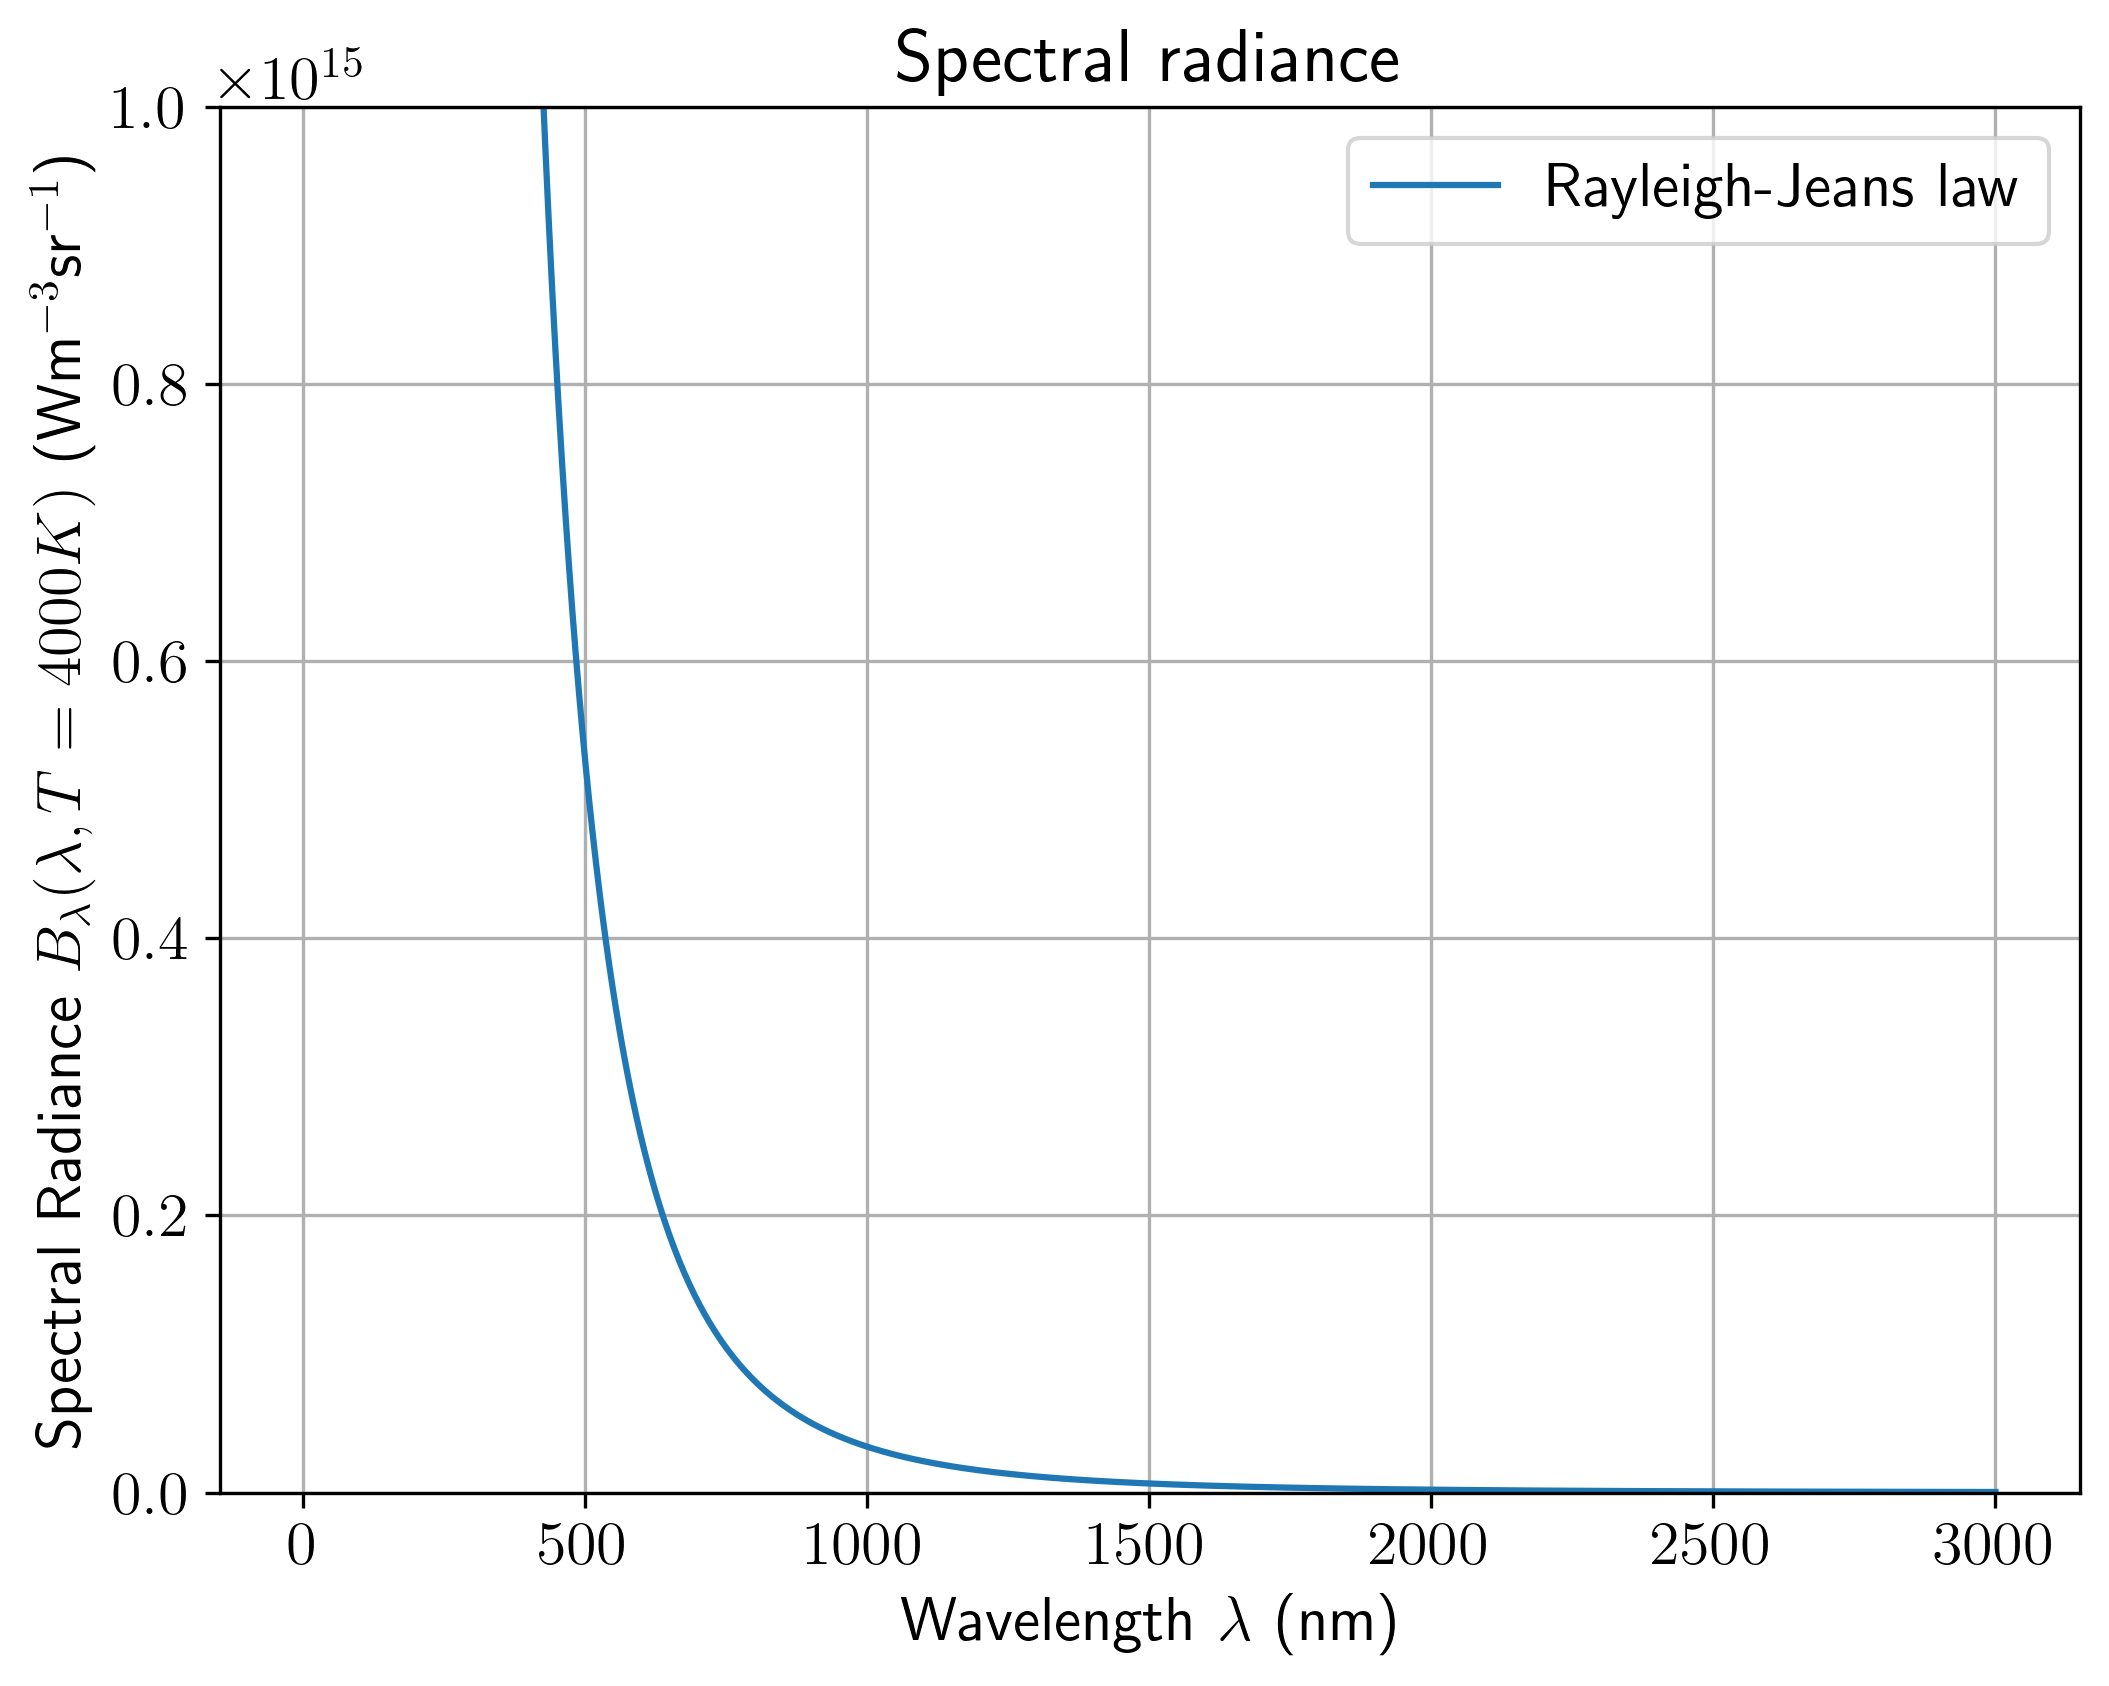
\includegraphics{SP1.1_-_Stellar_Properties_files/figure-pdf/cell-18-output-1.png}

}

\end{figure}

The Rayleigh-Jeans law has a big problem - the radiance keeps increasing
indefinitely at short wavelengths (higher frequencies). If it were true
the power emitted at short wavelengths would be infinite! This is known
as the Ultraviolet Catastrophe, and indicates the failure of classical
physics to explain the behaviour of thermal radiation.

\hypertarget{wiens-law}{%
\subsubsection{\texorpdfstring{7.2.2. \protect\hyperlink{toc0_}{Wien's
law}}{7.2.2. Wien's law}}\label{wiens-law}}

Wien's law is a good approximation to the observed spectrum at short
wavelength (high frequencies) \(hc\gg k_BT\lambda\).

\begin{align}
B_\lambda^\mathrm{Wien}(\lambda; T) = \frac{2 hc^2}{\lambda^5}\exp\left(-\frac{hc}{\lambda k_B T}\right)
\end{align}

\begin{Shaded}
\begin{Highlighting}[]
\NormalTok{B\_wien}\OperatorTok{=}\DecValTok{2} \OperatorTok{*}\NormalTok{ h.value }\OperatorTok{*}\NormalTok{c.value}\OperatorTok{**}\DecValTok{2} \OperatorTok{*}\NormalTok{ np.exp(}\OperatorTok{{-}}\NormalTok{h.value}\OperatorTok{*}\NormalTok{c.value}\OperatorTok{/}\NormalTok{((l}\OperatorTok{*}\FloatTok{1e{-}9}\NormalTok{)}\OperatorTok{*}\NormalTok{k\_B.value}\OperatorTok{*}\NormalTok{T)) }\OperatorTok{/}\NormalTok{ (l}\OperatorTok{*}\FloatTok{1e{-}9}\NormalTok{)}\OperatorTok{**}\DecValTok{5}\OperatorTok{;}
\end{Highlighting}
\end{Shaded}

\begin{Shaded}
\begin{Highlighting}[]
\NormalTok{plt.plot(l, B\_rj, label}\OperatorTok{=}\StringTok{"Rayleigh{-}Jeans law"}\NormalTok{)}
\NormalTok{plt.plot(l, B\_wien, label}\OperatorTok{=}\StringTok{"Wein\textquotesingle{}s law"}\NormalTok{)}

\NormalTok{plt.xlabel(}\VerbatimStringTok{r\textquotesingle{}Wavelength $\textbackslash{}lambda$ (nm)\textquotesingle{}}\NormalTok{)}
\NormalTok{plt.ylabel(}\VerbatimStringTok{r\textquotesingle{}Spectral Radiance $B\_\textbackslash{}lambda(\textbackslash{}lambda, T=4000K)$ (Wm$\^{}\{{-}3\}$sr$\^{}\{{-}1\}$)\textquotesingle{}}\NormalTok{)}
\NormalTok{plt.title(}\StringTok{\textquotesingle{}Spectral radiance\textquotesingle{}}\NormalTok{)}
\NormalTok{plt.ylim([}\DecValTok{0}\NormalTok{,}\FloatTok{5e12}\NormalTok{])}
\NormalTok{plt.grid()}
\NormalTok{plt.legend()}\OperatorTok{;}
\end{Highlighting}
\end{Shaded}

\begin{figure}[H]

{\centering 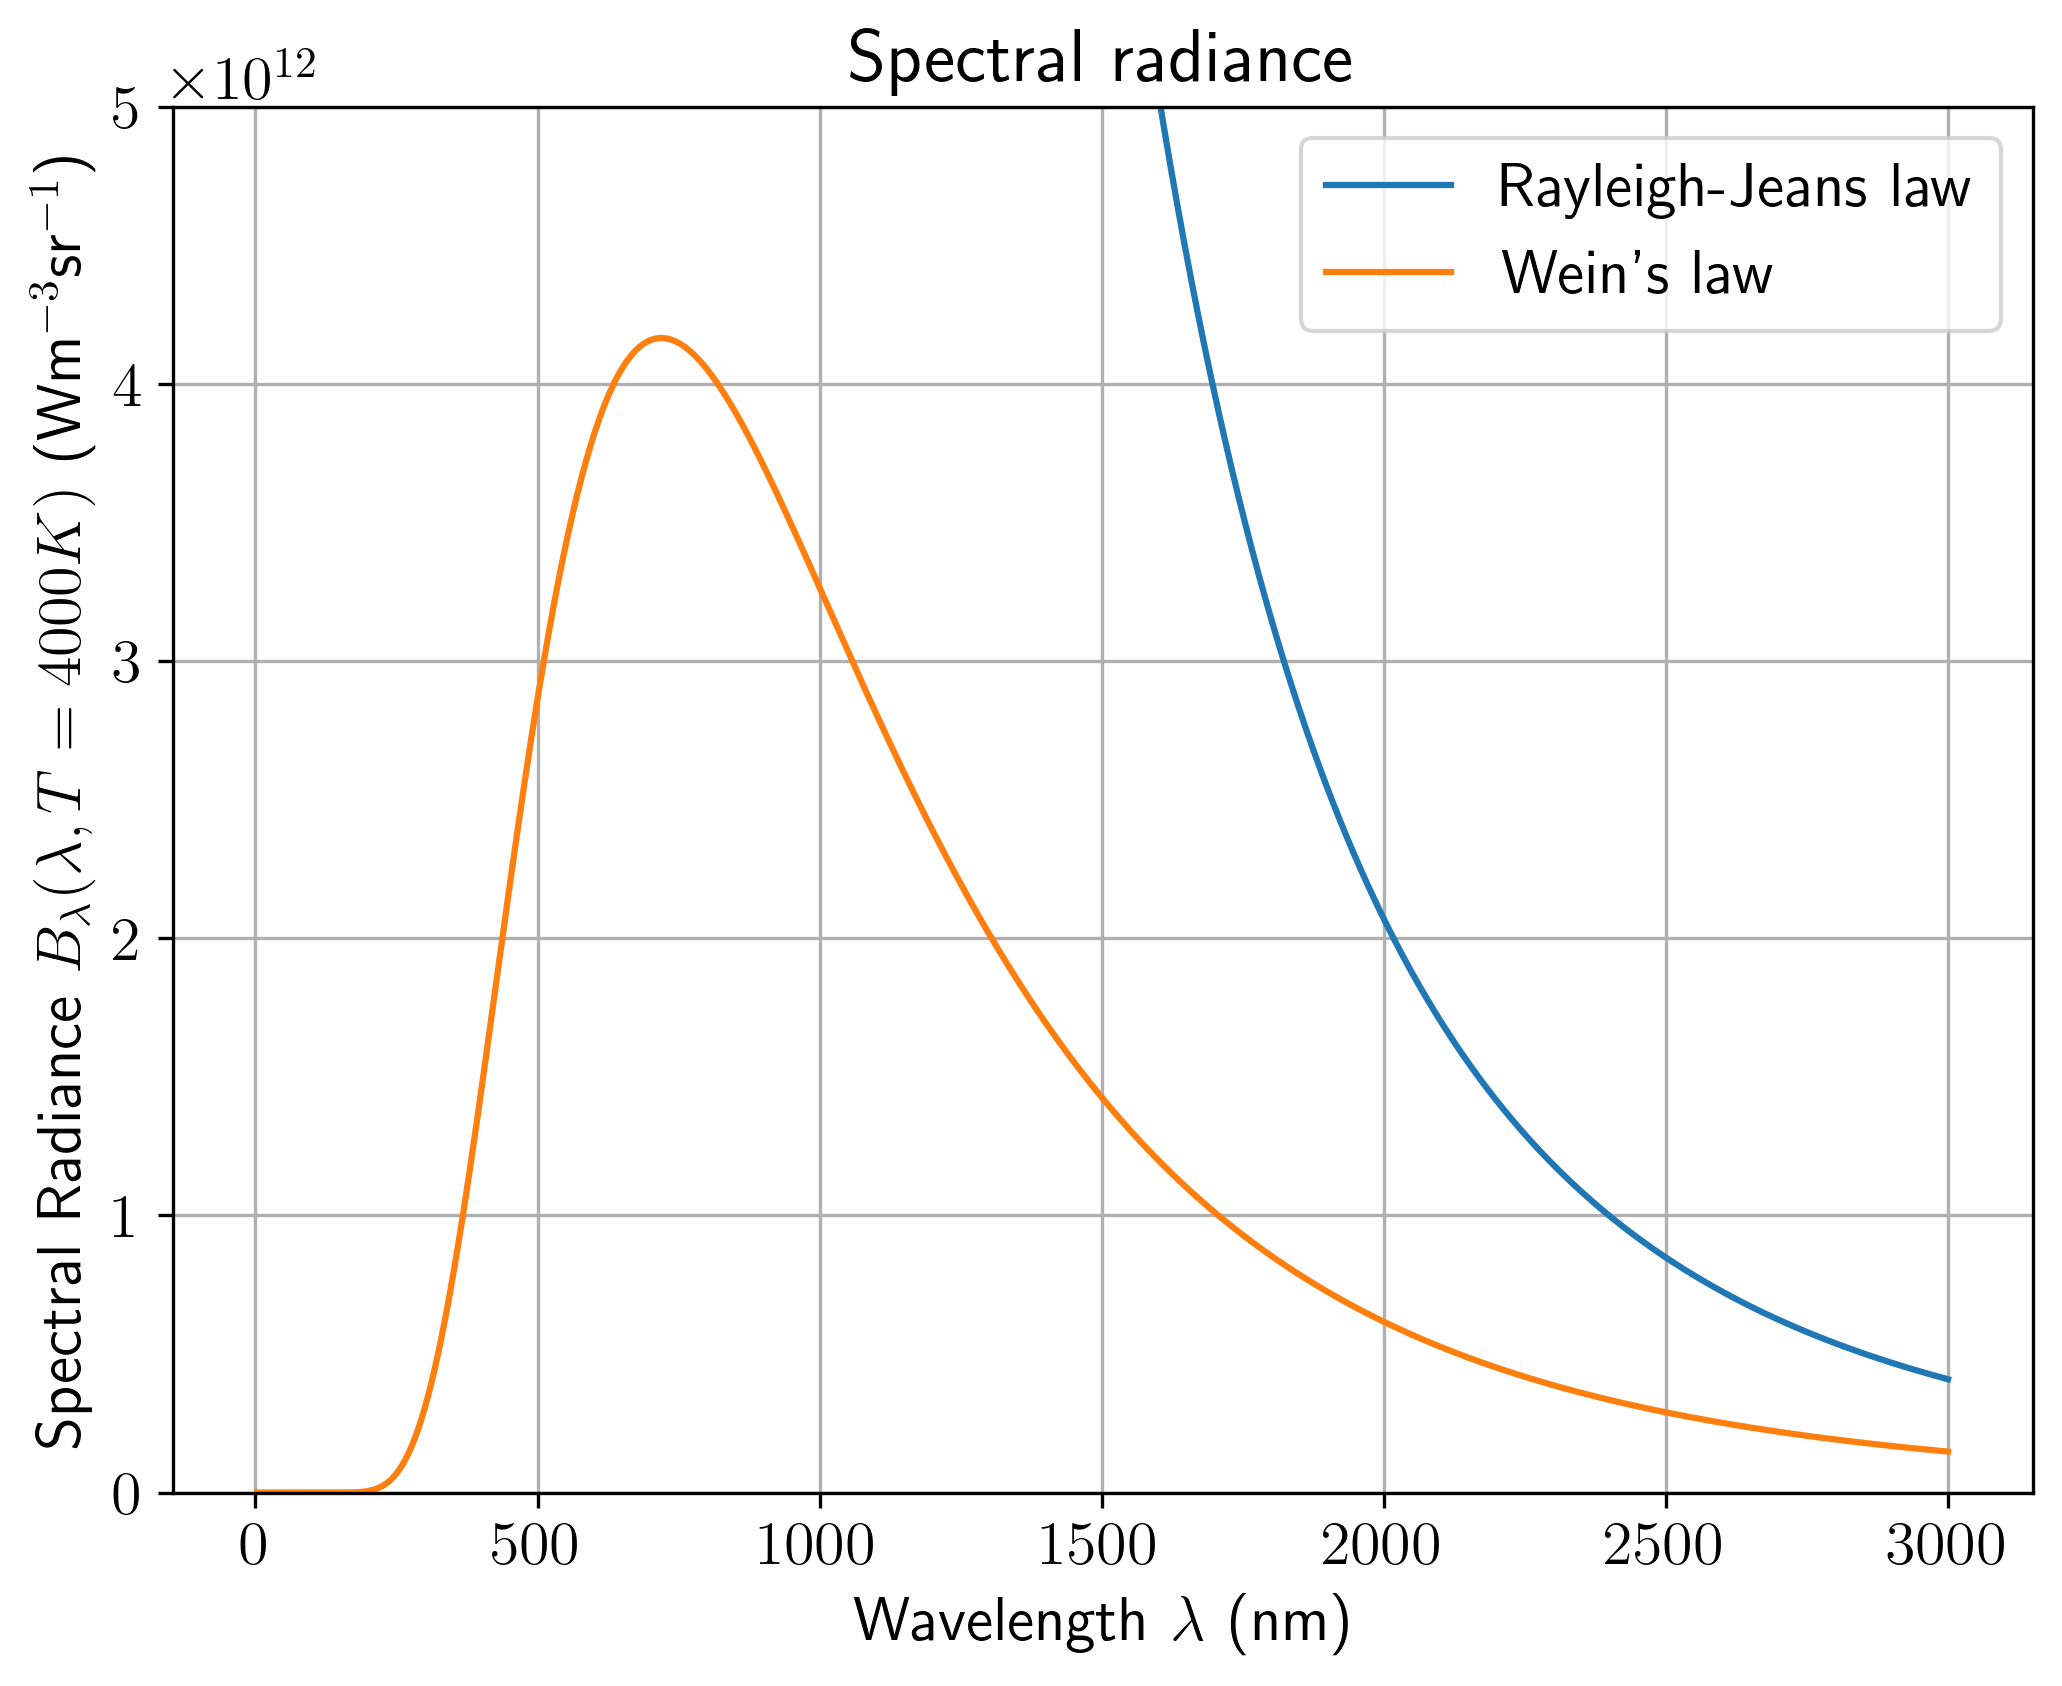
\includegraphics{SP1.1_-_Stellar_Properties_files/figure-pdf/cell-20-output-1.png}

}

\end{figure}

\hypertarget{plancks-law}{%
\subsection{\texorpdfstring{7.3. \protect\hyperlink{toc0_}{Planck's
Law}}{7.3. Planck's Law}}\label{plancks-law}}

In 1900, Planck was able to derive a spectrum that fit the data by
assuming that energy comes in discrete quanta. This marked the birth of
quantum physics! The Planck radiation spectrum for a black body's
spectral radiance is:

\begin{equation}
B_\lambda(\lambda; T) = \frac{2 hc^2}{\lambda^5}\left(\frac{1}{\exp\left(\frac{hc}{\lambda k_B T}\right) -1} \right)
\end{equation}

\begin{Shaded}
\begin{Highlighting}[]
\NormalTok{B\_planck }\OperatorTok{=} \DecValTok{2}\OperatorTok{*}\NormalTok{h.value}\OperatorTok{*}\NormalTok{c.value}\OperatorTok{**}\DecValTok{2} \OperatorTok{*}\NormalTok{ (}\FloatTok{1.0}\OperatorTok{/}\NormalTok{(np.exp(h.value}\OperatorTok{*}\NormalTok{c.value}\OperatorTok{/}\NormalTok{(k\_B.value}\OperatorTok{*}\NormalTok{T}\OperatorTok{*}\NormalTok{(l}\OperatorTok{*}\FloatTok{1e{-}9}\NormalTok{)))}\OperatorTok{{-}}\DecValTok{1}\NormalTok{)) }\OperatorTok{/}\NormalTok{ (l}\OperatorTok{*}\FloatTok{1e{-}9}\NormalTok{)}\OperatorTok{**}\DecValTok{5}\OperatorTok{;}
\NormalTok{plt.plot(l, B\_planck, label}\OperatorTok{=}\StringTok{"Planck\textquotesingle{}s law"}\NormalTok{)}
\NormalTok{plt.plot(l, B\_wien, label}\OperatorTok{=}\StringTok{"Wein\textquotesingle{}s law"}\NormalTok{)}
\NormalTok{plt.plot(l, B\_rj, label}\OperatorTok{=}\StringTok{"Rayleigh{-}Jeans law"}\NormalTok{)}

\NormalTok{plt.xlabel(}\VerbatimStringTok{r\textquotesingle{}Wavelength $\textbackslash{}lambda$ (nm)\textquotesingle{}}\NormalTok{)}
\NormalTok{plt.ylabel(}\VerbatimStringTok{r\textquotesingle{}Spectral Radiance $B\_\textbackslash{}lambda(\textbackslash{}lambda, T=4000K)$ (Wm$\^{}\{{-}3\}$sr$\^{}\{{-}1\}$)\textquotesingle{}}\NormalTok{)}
\NormalTok{plt.title(}\StringTok{\textquotesingle{}Spectral radiance\textquotesingle{}}\NormalTok{)}
\NormalTok{plt.ylim([}\DecValTok{0}\NormalTok{,}\FloatTok{5e12}\NormalTok{])}
\NormalTok{plt.grid()}
\NormalTok{plt.legend()}\OperatorTok{;}
\end{Highlighting}
\end{Shaded}

\begin{figure}[H]

{\centering 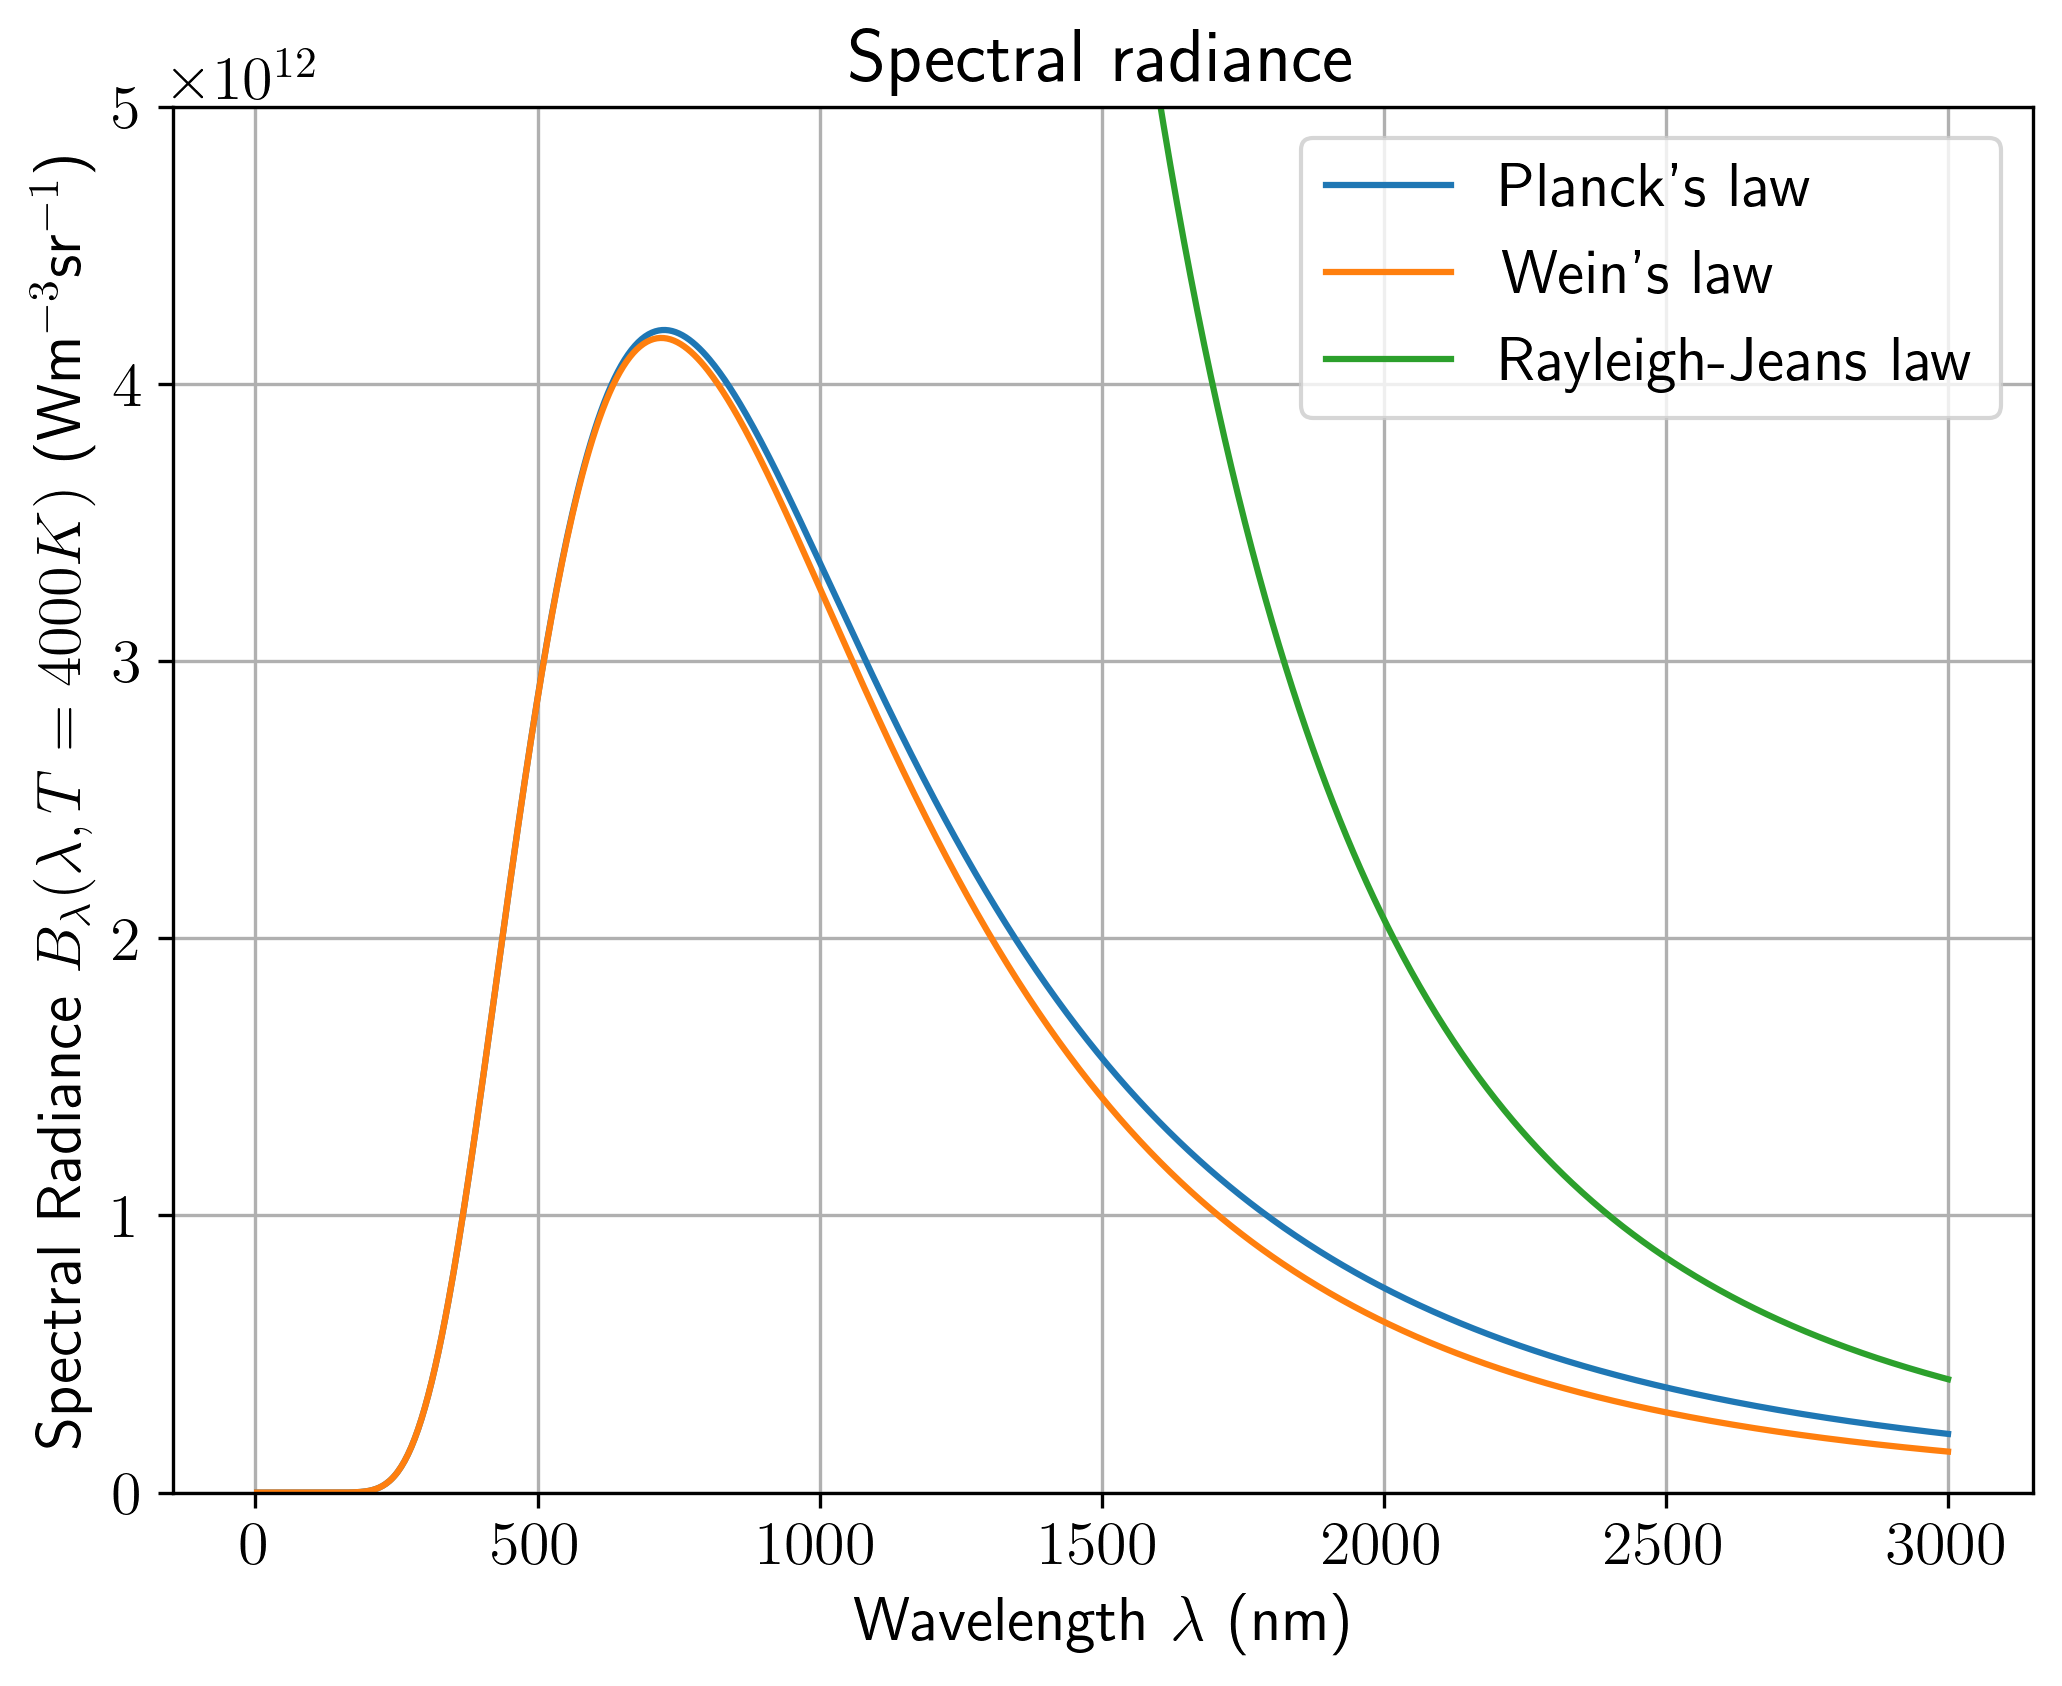
\includegraphics{SP1.1_-_Stellar_Properties_files/figure-pdf/cell-21-output-1.png}

}

\end{figure}

\hypertarget{exercise}{%
\subsubsection{\texorpdfstring{7.3.1.
\protect\hyperlink{toc0_}{Exercise:}}{7.3.1. Exercise:}}\label{exercise}}

\begin{enumerate}
\def\labelenumi{\arabic{enumi}.}
\tightlist
\item
  Show that for low frequencies (\(hc \ll \lambda k_B T\)) the
  Rayleigh-Jeans law can be derived from the Planck law.
\item
  Show that for high frequencies (\(hc \gg \lambda k_B T\)) Wein's law
  can be derived from the Planck law.
\end{enumerate}

You can use the approximation \(\lim_{x\rightarrow 0} \exp(x) = 1 + x\)

\hypertarget{temperature-and-colour}{%
\section{\texorpdfstring{8. \protect\hyperlink{toc0_}{Temperature and
colour}}{8. Temperature and colour}}\label{temperature-and-colour}}

Let's look at how the spectrum changes with temperature \(T\).

\begin{Shaded}
\begin{Highlighting}[]
\ControlFlowTok{for}\NormalTok{ T }\KeywordTok{in}\NormalTok{ [}\DecValTok{6000}\NormalTok{,}\DecValTok{5500}\NormalTok{,}\DecValTok{5000}\NormalTok{,}\DecValTok{4500}\NormalTok{,}\DecValTok{4000}\NormalTok{]:}
\NormalTok{    B\_planck }\OperatorTok{=} \DecValTok{2}\OperatorTok{*}\NormalTok{h.value}\OperatorTok{*}\NormalTok{c.value}\OperatorTok{**}\DecValTok{2} \OperatorTok{*}\NormalTok{ (}\FloatTok{1.0}\OperatorTok{/}\NormalTok{(np.exp(h.value}\OperatorTok{*}\NormalTok{c.value}\OperatorTok{/}\NormalTok{(k\_B.value}\OperatorTok{*}\NormalTok{T}\OperatorTok{*}\NormalTok{(l}\OperatorTok{*}\FloatTok{1e{-}9}\NormalTok{)))}\OperatorTok{{-}}\DecValTok{1}\NormalTok{)) }\OperatorTok{/}\NormalTok{ (l}\OperatorTok{*}\FloatTok{1e{-}9}\NormalTok{)}\OperatorTok{**}\DecValTok{5}
\NormalTok{    plt.plot(l, B\_planck, label}\OperatorTok{=}\StringTok{\textquotesingle{}T=\textquotesingle{}}\OperatorTok{+}\BuiltInTok{str}\NormalTok{(T)}\OperatorTok{+}\StringTok{\textquotesingle{}K\textquotesingle{}}\NormalTok{)}

\NormalTok{plt.xlabel(}\VerbatimStringTok{r\textquotesingle{}Wavelength $\textbackslash{}lambda$ (nm)\textquotesingle{}}\NormalTok{)}
\NormalTok{plt.ylabel(}\VerbatimStringTok{r\textquotesingle{}Spectral Radiance $B\_\textbackslash{}lambda(\textbackslash{}lambda, T=4000K)$ (Wm$\^{}\{{-}3\}$sr$\^{}\{{-}1\}$)\textquotesingle{}}\NormalTok{)}
\NormalTok{plt.title(}\StringTok{\textquotesingle{}Spectral radiance at different temperatures\textquotesingle{}}\NormalTok{)}
\NormalTok{plt.grid()}
\NormalTok{plt.legend()}\OperatorTok{;}
\end{Highlighting}
\end{Shaded}

\begin{figure}[H]

{\centering 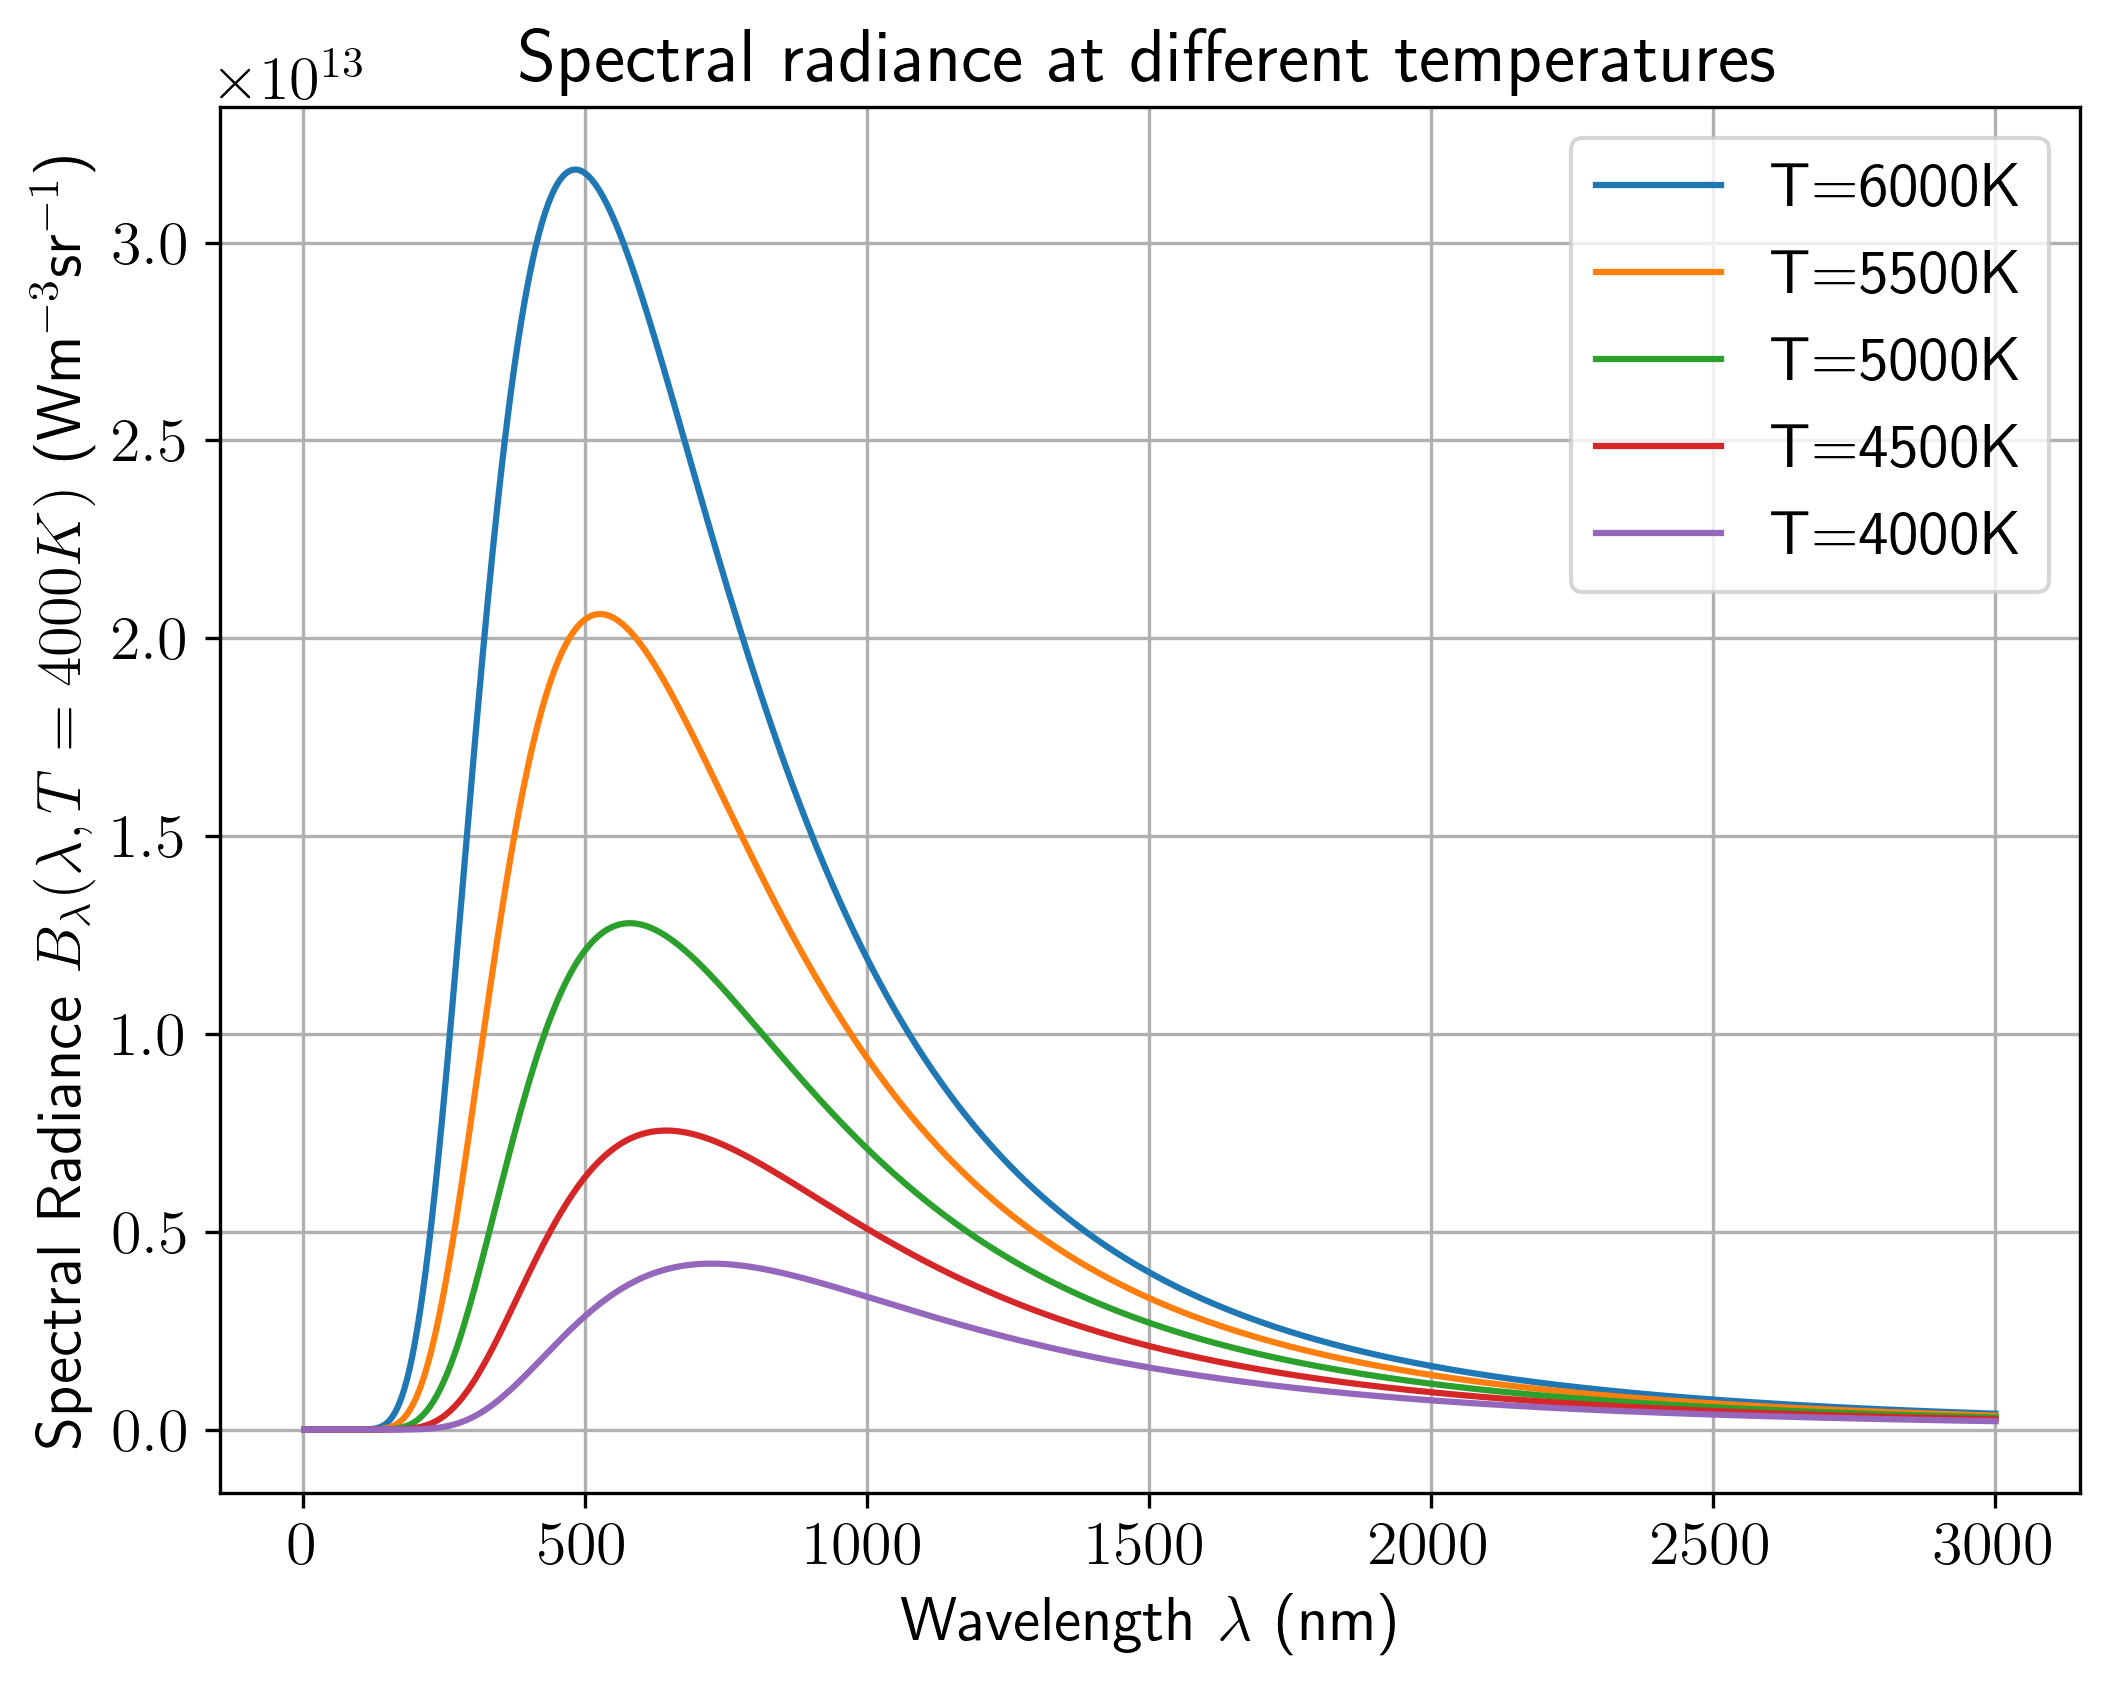
\includegraphics{SP1.1_-_Stellar_Properties_files/figure-pdf/cell-22-output-1.png}

}

\end{figure}

We notice that the Planck spectrum - has a clear peak at some
wavelength, which decreases as temperature increases -
\(B_\lambda(\lambda;T)> 0\) for all wavelengths, but tends toward \(0\)
at the extreme ends of the spectrum - overall increases with temperature

Black bodies radiate at all wavelengths - they won't look black! The
shape of the spectrum and the position of the peak determines the
apparent colour of the object.

\hypertarget{wiens-displacement-law}{%
\subsection{\texorpdfstring{8.1. \protect\hyperlink{toc0_}{Wien's
displacement
law}}{8.1. Wien's displacement law}}\label{wiens-displacement-law}}

There is an inverse relationship between the temperature \(T\) in kelvin
and the peak emission wavelength \(\lambda_{peak}\) in metres, called
Wien's displacement law: \begin{align}
\lambda_{peak} = \frac{0.0029\,\mathrm{m\,K}}{T}
\end{align}

Where \(\mathrm{m\,K}\) are metres \(\times\) kelvin, the units of the
constant.

We can use this to determine the effective temperature of a star from
the spectrum of its light, assuming it is a black body.

\hypertarget{example-2}{%
\subsection{\texorpdfstring{8.2.
\protect\hyperlink{toc0_}{Example}}{8.2. Example}}\label{example-2}}

The Sun's spectrum has a peak wavelength of around 500 nm, in the green
part of the spectrum.

What is the effective emission temperature of the Sun?

\begin{Shaded}
\begin{Highlighting}[]
\NormalTok{w }\OperatorTok{=} \FloatTok{0.0029} \CommentTok{\# constant}
\NormalTok{lmax }\OperatorTok{=} \FloatTok{501e{-}9} \CommentTok{\# peak wavelength in metres}
\NormalTok{Tsun }\OperatorTok{=}\NormalTok{ w}\OperatorTok{/}\NormalTok{lmax}
\BuiltInTok{print}\NormalTok{(}\StringTok{\textquotesingle{}The effective temperature of the Sun is }\SpecialCharTok{\{0\}}\StringTok{ K\textquotesingle{}}\NormalTok{.}\BuiltInTok{format}\NormalTok{(Tsun))}
\end{Highlighting}
\end{Shaded}

\begin{verbatim}
The effective temperature of the Sun is 5788.423153692614 K
\end{verbatim}

The commonly used value is \(T_\odot=5780\) K

Although the peak emission is greenish, the distribution overall
produces light that appears yellowish to us, after passing throught the
atmosphere.

\hypertarget{converting-between-wavelength-and-frequency}{%
\subsection{\texorpdfstring{8.3. \protect\hyperlink{toc0_}{(!)
Converting between wavelength and
frequency}}{8.3. (!) Converting between wavelength and frequency}}\label{converting-between-wavelength-and-frequency}}

So far we have been using the spectral radiance in terms of wavelength
\(B_\lambda(\lambda;T)\). It can also be expressed in terms of the
frequency of the radiation \(B_\nu(\nu;T)\). Since it is a density
across wavelengths, we must be careful when converting between them.

\begin{align}
B_\nu(\nu;T)d\nu &= B_\lambda(\lambda;T)d\lambda \\
B_\nu(\nu;T) &= B_\lambda(\lambda(\nu);T) \left|\frac{d\lambda}{d\nu}\right| \\
 &= B_\lambda(c/\nu; T) \left|-\frac{c}{\nu^2}\right| \\
  &= \frac{2h\nu^5}{c^3}\left( \frac{1}{\exp\left(\frac{h\nu}{k_BT}\right)-1} \right) \times \frac{c}{\nu^2} \\
  B_\nu(\nu;T) &= \frac{2h\nu^3}{c^2}\left( \frac{1}{\exp\left(\frac{h\nu}{k_BT}\right)-1}\right)
\end{align}

\hypertarget{okay-but-how-big-is-an-a.u.}{%
\subsection{\texorpdfstring{8.4. \protect\hyperlink{toc0_}{Okay, but how
big is an
a.u.?}}{8.4. Okay, but how big is an a.u.?}}\label{okay-but-how-big-is-an-a.u.}}

In 1976 the International Astronomical Union (IAU) adopted a standard
definition whose value has been updated with increasing precision during
the years. At the current date, the astronomical unit is: - 1 a.u. =
149,597,870,700 m

\hypertarget{are-stars-really-black-bodies}{%
\subsection{\texorpdfstring{8.5. \protect\hyperlink{toc0_}{Are stars
really black
bodies?}}{8.5. Are stars really black bodies?}}\label{are-stars-really-black-bodies}}

\begin{itemize}
\tightlist
\item
  The Planck black body spectrum is a theoretical prediction for an
  ideal case.
\item
  Light from the Sun is obscured by the atmosphere of the Earth, which
  absorbs some wavelengths more than others. This is called
  \emph{atmospheric extinction}. We will ignore this effect in this
  course.
\item
  There are also \emph{spectral lines}, gaps in the solar spectrum. More
  on this later.
\end{itemize}

\hypertarget{stefan-boltzmann-law}{%
\section{\texorpdfstring{9. \protect\hyperlink{toc0_}{Stefan-Boltzmann
Law}}{9. Stefan-Boltzmann Law}}\label{stefan-boltzmann-law}}

The total (bolometric) luminosity per area (``radiant emittance''
\(j=\frac{L}{A}\)) has units of \(\mathrm{W\,m}^{-2}\), and is the
spectral radiance integrated over solid angle and wavelength:

The equation for this is known as the Stefan-Boltzmann Law.
\begin{align}
j &= \frac{\pi^2 k_B^4 T^4}{60 \hbar^3 c^2}
\end{align}

This can be written more simply as

\begin{align}
j = \sigma T^4
\end{align}

where
\(\sigma = \frac{\pi^2 k_B^4 }{60 \hbar^3 c^2} = 5.67\times 10^{-8}\mathrm{W\,m^{-2}K^{-4}}\)
is the Stefan-Boltzmann constant.

\hypertarget{stellar-luminosity}{%
\section{\texorpdfstring{10. \protect\hyperlink{toc0_}{Stellar
luminosity}}{10. Stellar luminosity}}\label{stellar-luminosity}}

We can multiply by the surface area to find the total luminosity of a
spherical star of radius \(R\):

\begin{align}
L = 4\pi R^2 \sigma T^4
\end{align}

This is the most useful form to use in stellar calculations -
\textbf{remember it}!

It allows us to relate \(R\), \(L\), and \(T\) for a star.

\begin{itemize}
\tightlist
\item
  If we know the apparent magnitude and the distance \(d\), then we can
  find the absolute magnitude
\item
  If we know the absolute magnitude we can find the luminosity
\item
  If we know the luminosity and the temperature we can find the star's
  radius!
\end{itemize}

You need to be able to solve these types of problem - \textbf{practice
it}!

\hypertarget{example-3}{%
\subsection{\texorpdfstring{10.1.
\protect\hyperlink{toc0_}{Example}}{10.1. Example}}\label{example-3}}

\(\epsilon\)-Eridani is a star at \(r=3.212\) parsecs distance, with an
apparent bolometric magnitude of 3.54 and a peak emission wavelength of
570 nm. What else can we tell about it?

\begin{itemize}
\tightlist
\item
  Work out the absolute bolometric magnitude from the apparent
  bolometric magnitude
\end{itemize}

\begin{align}
M_\epsilon &= m_\epsilon + 5 - 5\log_{10}r \\
  &= 3.54 + 5 - 5\log_{10}(3.2) \\
  &= 6.0
\end{align}

\begin{itemize}
\tightlist
\item
  Work out the Luminosity from that and the distance
\item
  Remember solar absolute bolometric magnitude is 4.83
\end{itemize}

\begin{align}
M_{\epsilon} &= -2.5\log_{10}L_\epsilon+2.5\log_{10}L_\odot + 4.83 \\
2.5\log_{10}(L_\epsilon / L_\odot) &= 4.83 - M_\epsilon \\
&= 4.83 - 6.0  \\
&= -1.17 \\
\log_{10}(L_\epsilon / L_\odot) & = -0.468 \\
L_\epsilon / L_\odot &= 10^{-0.468} \\
\hline \\
L_\epsilon &= 0.34\,L_\odot \\
&= 1.3\times 10^{26}\,\mathrm{W}
\end{align}

\begin{itemize}
\tightlist
\item
  Work out the temperature using Wien's displacement law
\end{itemize}

\begin{align}
\lambda_{peak} T_\epsilon &= 0.0029 \\
T_\epsilon &= \frac{0.0029}{ 570\times 10^{-9}} \\
\hline \\
T_\epsilon &= 5088\,\mathrm{K}
\end{align}

\begin{itemize}
\tightlist
\item
  Work out the radius
\end{itemize}

\begin{align}
L_\epsilon &= 4\pi R_\epsilon^2 \sigma T^4 \\
R_\epsilon^2 &= \frac{L_\epsilon}{4\pi \sigma T^4} \\
R_\epsilon &= \sqrt{\frac{L_\epsilon}{4\pi \sigma T^4}} \\
&= \sqrt{\frac{1.3\times 10^{26}}{4\pi \times 5.671\times10^{-8}\times 5088^4}}  \\
\hline \\
&= 5.22\times 10^{9}\,\mathrm{m}
\end{align}

\hypertarget{recap-1}{%
\section{\texorpdfstring{11.
\protect\hyperlink{toc0_}{Recap}}{11. Recap}}\label{recap-1}}

\begin{itemize}
\tightlist
\item
  \textbf{Planck radiation law} gives the shape of the black-body
  emission spectrum
\item
  \textbf{Wien's displacement law} relates the peak emission wavelength
  to the temperature
\item
  \textbf{Stefan-Boltzmann law} can be used to find the total power
  radiated by a black body
\end{itemize}



\end{document}
